\documentclass[12pt,fleqn,a4paper,nodisplayskipstretch]{article}
\usepackage[utf8]{inputenc}
\usepackage[a4paper, left=30mm, right=20mm, top=30mm, bottom=20mm]{geometry}
\usepackage{ragged2e}
\usepackage{mathptmx}

\usepackage{fancyhdr}
\usepackage{quoting}
\usepackage{nomencl}
\usepackage[brazil]{babel}



\usepackage{bezier,amstext,amsthm,makeidx,indentfirst,ifthen,cite,minitoc}

\usepackage[]{setspace}

\usepackage[alf,abnt-repeated-title-omit=yes,abnt-emphasize=bf,abnt-etal-list=0]{abntex2cite}


\citebrackets()
\makenomenclature

\renewcommand{\footnoterule}{
\kern -3pt
\hrule width 5cm
\kern 2pt
}

\AtBeginDocument{
    %Centralização do título sumário
    \renewcommand\contentsname{\centering \normalsize \uppercase{Sumário}}
    %Renomeação do título das siglas
    \renewcommand{\nomname}{\centering \normalsize \uppercase{Siglas}} 
    %Remoção do título referências
    \renewcommand{\refname}{} 
    %Renomeação do título da lista de figuras
    \renewcommand{\listfigurename}{\centering \normalsize \uppercase{Lista de figuras}}
    %Renomeação do título da lista de tabela
    \renewcommand{\listtablename}{\centering \normalsize \uppercase{Lista de tabela}}
}

\pagestyle{fancy}
\fancyhf{}
\fancyheadoffset{0cm}
\renewcommand{\headrulewidth}{0pt} 
\renewcommand{\footrulewidth}{0pt}
\fancyhead[R]{\thepage}
\fancypagestyle{plain}{
  \fancyhf{}
  \fancyhead[R]{\thepage}
}


\begin{document}
\pagestyle{empty}
\begin{center}
\bf{Universidade Estadual Paulista ``Júlio de Mesquita Filho''}
  
  \bf{FCT — Faculdade de Ciências e Tecnologia}
  
  \bf{DMC — Departamento de Matemática e Computação}
  
  \bf{Bacharelado em Ciência da Computação}
  
  \vspace*{\fill}
  \vspace{42pt}
  \Large{	\textmd{Trabalho de Conclusão de Curso}}
    
  \large{Anteprojeto de pesquisa}
  
  \vspace{42pt}
  \Large{Aplicação de métodos de Inpainting em imagens digitais}
  
  \vspace{42pt}
  \normalsize{\bf{Gustavo Becelli do Nacimento}
  
  \vspace{12pt}
  Orientador: \textmd{Prof.\ Dr.\ Almir Olivette Artero}}
  
  \vspace*{\fill}
  \vspace{12pt}
  Presidente Prudente, 22 de janeiro de 2023
\end{center}
\pagebreak

\pagestyle{empty}
\tableofcontents{}
\pagebreak

% \section*{Resumo}
O inpainting de imagens é a técnica de modificar imagens com aplicação majoritariamente concentrada em restauração de imagens corrompidas por ruídos, borrões, arranhões, objetos indesejados, textos sobrepostos (e.g. legendas e marcas-d’-água), defeitos da lente de captura, entre diversas outras falhas em imagens digitais. 

Os métodos estabelecidas para aplicar o inpainting podem ser divididos em duas categorias: (1) métodos sequenciais clássicos, e (2) métodos baseados em aprendizado, que utilizam redes neurais convolucionais (CNNs) e/ou Redes Generativas Adversárias (GANs). A primeira categoria ordinariamente possui métodos mais leves, que recorrem às equações diferenciais parciais (PDEs), enquanto as duas últimas, para obterem melhores resultados, utilizam maior processamento computacional e necessitam de treinamento prévio para ajustar seus parâmetros.

Este trabalho desenvolverá este tema e apresentará uma revisão teórica dos métodos de inpainting, aprentado algumas das técnicas e conceitos principais utilizados. Como resultado, foi possível compreender que os métodos clássicos são, em geral, mais rápidos e eficientes, mas apresentam resultados menos realistas e borramentos. Por outro lado, os métodos baseados em aprendizado são mais lentos e computacionalmente mais custosos, mas apresentam resultados mais plausíveis. Apesar disto, em geral, todos costumam considerar as regiões vizinhas ou semelhantes para preencher a região alvo.

Palavras-chave: Inpainting, processamento de imagens, preenchimento de regiões, aprendizado de máquina.
\pagebreak
\section*{Abstract}
Image inpainting is a technique for modifying images with application mainly focused on restoring images corrupted by noise, blurs, scratches, unwanted objects, superimposed texts (e.g. subtitles and watermarks), capture lens defects, among others. several other flaws in digital images.

The established methods for applying inpainting can be divided into two categories: (1) classical sequential methods, and (2) learning-based methods, which use convolutional neural networks (CNNs) and/or Generative Adversarial Networks (GANs). The first category ordinarily has lighter methods, which resort to partial differential equations (PDEs), while the last two, in order to obtain better results, use more computational processing and require prior training to adjust their parameters.

This work will develop this theme and present a theoretical review of inpainting methods, presenting some of the techniques and main concepts used. As a result, it was possible to understand that the classical methods are, in general, faster and more efficient, but present less realistic results and blurring. On the other hand, learning-based methods are slower and computationally more expensive, but present more plausible results. Despite this, in general, everyone usually considers neighboring or similar regions to fill the target region.

Keywords: Inpainting, image processing, region filling, machine learning.
% \pagebreak

\pagenumbering{arabic}
% Apresentar uma panorâmica da área a ser estudada, descrevendo o histórico da área, o cenário atual, os problemas existentes, o objetivo deste trabalho e, no final, a estrutura deste documento, descrevendo brevemente os demais capítulos desta revisão.

\section{Introdução} \label{introduction}
O Inpainting  de Imagens é o processo de preencher regiões faltantes ou danificadas de uma imagem com o intuito de restaurá-la ou melhorar sua aparência. Este é um problema amplamente estudado em visão computacional e possui uma vasta gama de oportunidades de aplicações, incluindo o restauro de obras artísticas e fotografias danificadas, a remoção de objetos de imagens e síntese de texturas~\cite{criminisi2004region}.

Esta área de pesquisa tem sido estudada há várias décadas. Os primeiros trabalhos sobre o tema surgiram na década de 1950, mas foi somente a partir dos anos 1990 que o inpainting começou a ser utilizado de maneira mais ampla.

\cite{Elharrouss2019} apresenta uma revisão sobre o inpainting de imagens, descrevendo os principais métodos e aplicações. Neste campo, existem várias técnicas para o inpainting de imagens, cada tal com suas próprias vantagens e desvantagens. Uma abordagem popular é apresentada em \cite{Bertalmio2000}, a qual introduz uma técnica de inpainting baseada no conceito de complementar uma região de uma imagem existente. Neste trabalho é utilizado equações diferenciais parciais para propagar informações das bordas da região danificada para o centro da região, permitindo que o algoritmo estime como os pixels devem ser restaurados.

Uma das contribuições mais significativas para o campo de inpainting de imagem é o desenvolvimento do ``Método de Marcha Rápida'' ~\cite{Telea2004}, um algoritmo eficiente que usa equações diferenciais parciais para propagar informações de pixels conhecidos para os pixels desconhecidos na região de inpainting. Este algoritmo tem sido amplamente utilizado em várias aplicações e foi implementado em muitas bibliotecas de software, incluindo a biblioteca de código aberto de visão computacional OpenCV \cite{OpenCV}. Este método tem demonstrado produzir resultados de alta qualidade para uma ampla variedade de tipos de imagem e cenários, e se tornou uma das referências para avaliar o desempenho de outros algoritmos de inpainting.

Nos últimos anos, houve um aumento de interesse em utilizar métodos baseados em aprendizado de máquina, como redes adversárias gerativas (GANs) e redes neurais convolucionais (CNNs) \cite{pathakCVPR16context}, para resolver o problema de inpainting. Esses métodos têm o potencial de aprender padrões e estruturas complexas a partir de grandes conjuntos de dados, o que pode ser usado para gerar resultados de inpainting de alta qualidade. No entanto, esses métodos podem ser computacionalmente caros e podem exigir uma abundância de dados de treinamento para obter bons resultados.

Hoje, o inpainting é utilizado em uma variedade de aplicações. Dentre elas, está incluída o restauro de obras de arte danificadas, a remoção de objetos de imagens (como nuvens em imagens de sensoriamento remoto) e até mesmo a
remoção de imperfeições de fotografias. Além disso, pode-se utilizar os mesmos conceitos de restauração para modificar as perspectivas de imagens, como é apresentado em \cite{huang2014image}.

O principal problema encontrado neste campo de pesquisa são a escolha do método de inpainting mais adequado para cada tipo de imagem e cenário. Este fator se deve às desvantagens que os métodos existentes proporcionam \cite{Salem2021}. Em geral, os maiores desafios são:
\begin{itemize} 
  \item \textbf{Preservação da consistência e estrutura da imagem de entrada:} muitos modelos geradores podem gerar imagens visualmente agradáveis, mas que não correspondem perfeitamente com a vizinhança ou à textura da imagem original.
  \item \textbf{Preservação de pequenos detalhes:} este problema é particularmente desafiador para imagens com texturas complexas, como imagens de paisagens naturais, ou a área que está sendo restaurada é muito grande.
  \item \textbf{Reconstruir objetos sobrepostos:} quando um objeto é parcial ou completamente sobreposto, como um objeto que está coberto por uma nuvem, o modelo gerador pode não ser capaz de reconstruir o objeto original.
  \item \textbf{Preenchimento de grandes regiões:} a geração de imagens de alta qualidade quando há uma grande região a ser reconstruída ainda é um problema desafiador.
  \item \textbf{Desempenho computacional:} a maioria dos métodos de inpainting de imagens que geram imagens de alta qualidade são computacionalmente caros, dificultando sua aplicação em tempo real.
\end{itemize}


\subsection{Objetivos}

\subsubsection{Objetivo principal}
O objetivo principal deste Trabalho de Conclusão de Curso é investigar e implementar algumas das diferentes técnicas de Inpainting para a restauração de imagens digitais com defeitos ou objetos indesejados. Para alcançar esse objetivo, serão estudadas técnicas clássicas baseadas em informações de vizinhança e amostras, bem como técnicas mais recentes baseadas em aprendizado de máquina. Além disso, serão aplicadas as técnicas estudadas em diversos tipos de imagens para avaliar sua eficácia e comparar os resultados obtidos.

\subsubsection{Objetivos secundários}
\begin{itemize}
  \item Estudar alguns dos principais métodos de inpainting, com o intuito de entender como cada um deles funciona e quais são suas vantagens e desvantagens.
  \item Aplicar as técnicas de inpainting estudadas em diversos tipos de imagens, incluindo imagens coloridas, imagens de alta resolução e imagens com diferentes tipos de defeitos, como buracos, riscos, manchas, etc.
  \item Aperfeiçoar os conhecimentos em processamento de imagens e aprendizado de máquina do aluno, bem como a capacidade de aplicar esses conhecimentos em problemas reais.
  \item Estudar a possibilidade de melhorias na eficácia (qualidade das imagens geradas) e na eficiência (tempo de processamento, uso de memória) dos métodos de inpainting estudados.
\end{itemize}

Os três objetivos secundários representam o âmbito deste trabalho dentro do objetivo principal. O último, por sua vez, representa o interesse do aluno em aprofundar seus conhecimentos em otimização computacional de algoritmos e a possibilidade de contribuir com a comunidade científica.

\subsection{Organização do Trabalho}
Inicialmente apresenta-se uma fundamentação teórica sobre o processo de inpainting, incluindo uma breve introdução sobre o escopo de inpainting, as principais categorias da área e posteriormente uma revisão de alguns dos principais métodos utilizados.
Em seguida, há uma seção destinada a mencionar algumas possíveis técnicas de otimização computacionais que podem ser aplicadas caso haja a possibilidade de serem implementadas.

Por fim, é apresentado um 
\pagebreak

% \section{Trabalhos Relacionados} \label{related}

A Tabela \ref{related-works} apresenta, de forma resumida, os principais trabalhos relacionados ao tema deste trabalho, apresentando os seus objetivos, métodos e resultados.

% Referência | ano | Objetivo | Método | Resultado
% do not overflow the page width.
% break lines if necessary.
% use tabularx environment
\begin{table}[h]
\centering
\caption{Trabalhos relacionados ao tema deste trabalho.}
\label{related-works}
\begin{tabularx}{\linewidth}{|l|l|X|X|X|}
\hline
\textbf{Referência} & \textbf{Ano} & \textbf{Objetivo} & \textbf{Método} & \textbf{Resultado} \\
\hline
\cite{Bertalmio2000} & 2000 & Inpainting de imagens com texturas e estruturas simples. & Patch-based. & Imagens com texturas e estruturas simples. \\


\hline

\end{tabularx}
\end{table}








% \input{method.tex}
% \section{Resultados obtidos}\label{sec:results}
Nesta seção serão apresentados dois problemas inclusos em um PVI que possuem solução analítica conhecida. Ambos abordam funções logísticas e possuem comportamento semelhante. O terceiro problema trata de um sistema fechado contendo populações de duas espécies que coexistem e exercem uma relação biológica não-harmônica.

\subsection{Primeiro problema: evolução dos casos de contaminação por uma doença} \label{problem-1}\quad
Considere o PVI adaptado de \cite{zill2001} a seguir:
\begin{equation}\label{pvi-ex1}
	\begin{cases}
		\frac{dy}{dt} = kt(1000-t) &                            \\
		y(0) = 1                   & \text{ com } t \in [0, 12] 
	\end{cases}
\end{equation}

onde:
\begin{itemize}
\item $y$ é o número de indivíduos infectados;
\item $k$ é a constante de decaimento do problema;
\item $t$ é a variável de tempo, medida em dias.
\end{itemize}

Neste exemplo, considera-se um PVI que descreve a evolução de uma doença respiratória leve que se espalha subitamente por uma população de $1000$ indivíduos ao longo de um período de 12 dias, começando com apenas um indivíduo infectado. Essa doença é transmitida assintomaticamente e não é fatal.

Seja $k = 9.906 \times 10^{-4}$ uma constante obtida de forma empírica, a solução de (\ref{pvi-ex1}) é dada por:
\begin{equation*}
	y(t) =  \dfrac{1000}{1 + 999e^{-1000kt}} = \dfrac{1000}{1 + 999e^{-0.9906t}}
\end{equation*}

A solução numérica, para todos os métodos estudados, pode ser visualizado na Figura \ref{img:ex1_plots}.

\begin{figure}[H]
	\centering
	\mbox{
		\subfigure[]{
			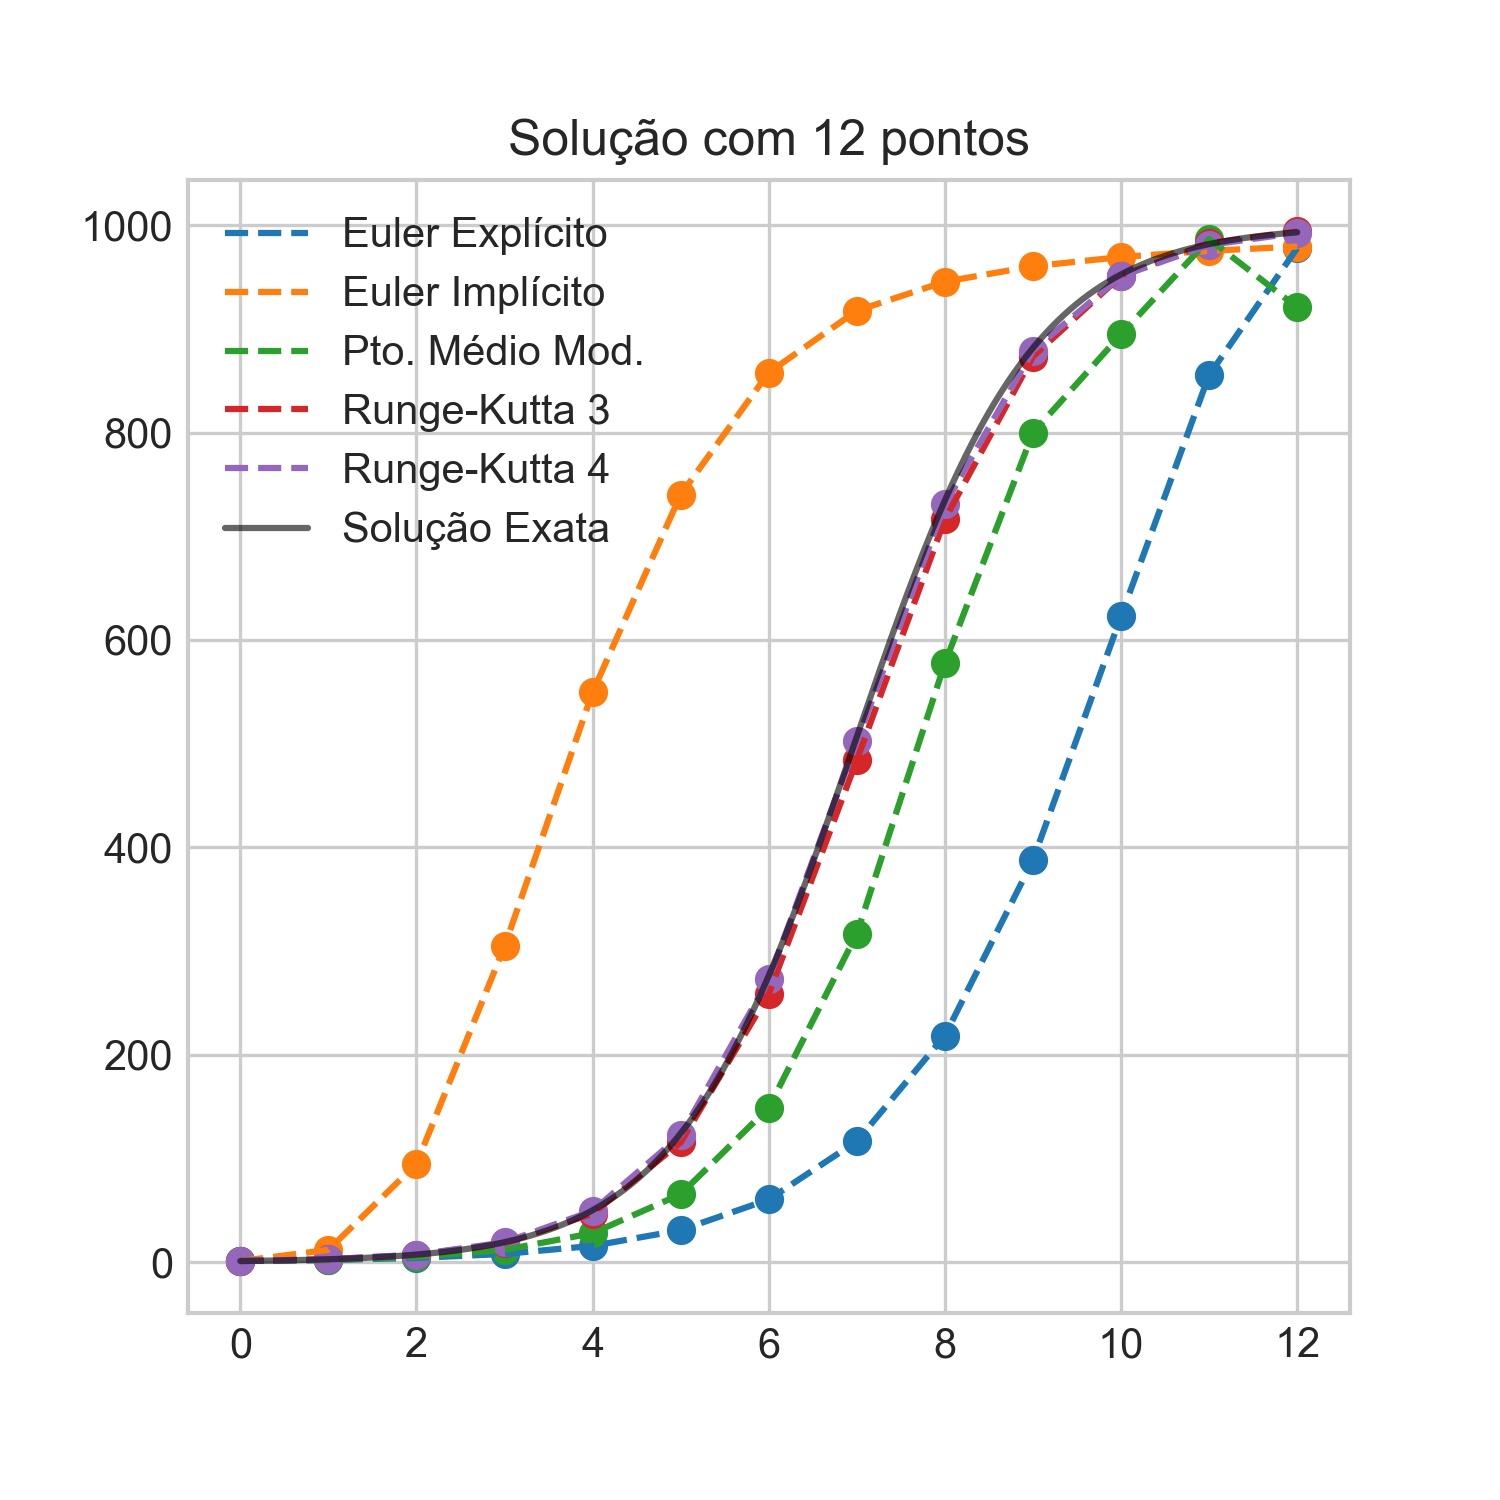
\includegraphics[height=7.8cm, width=7.8cm]{disease/solution_12.png}}
		\subfigure[]{
			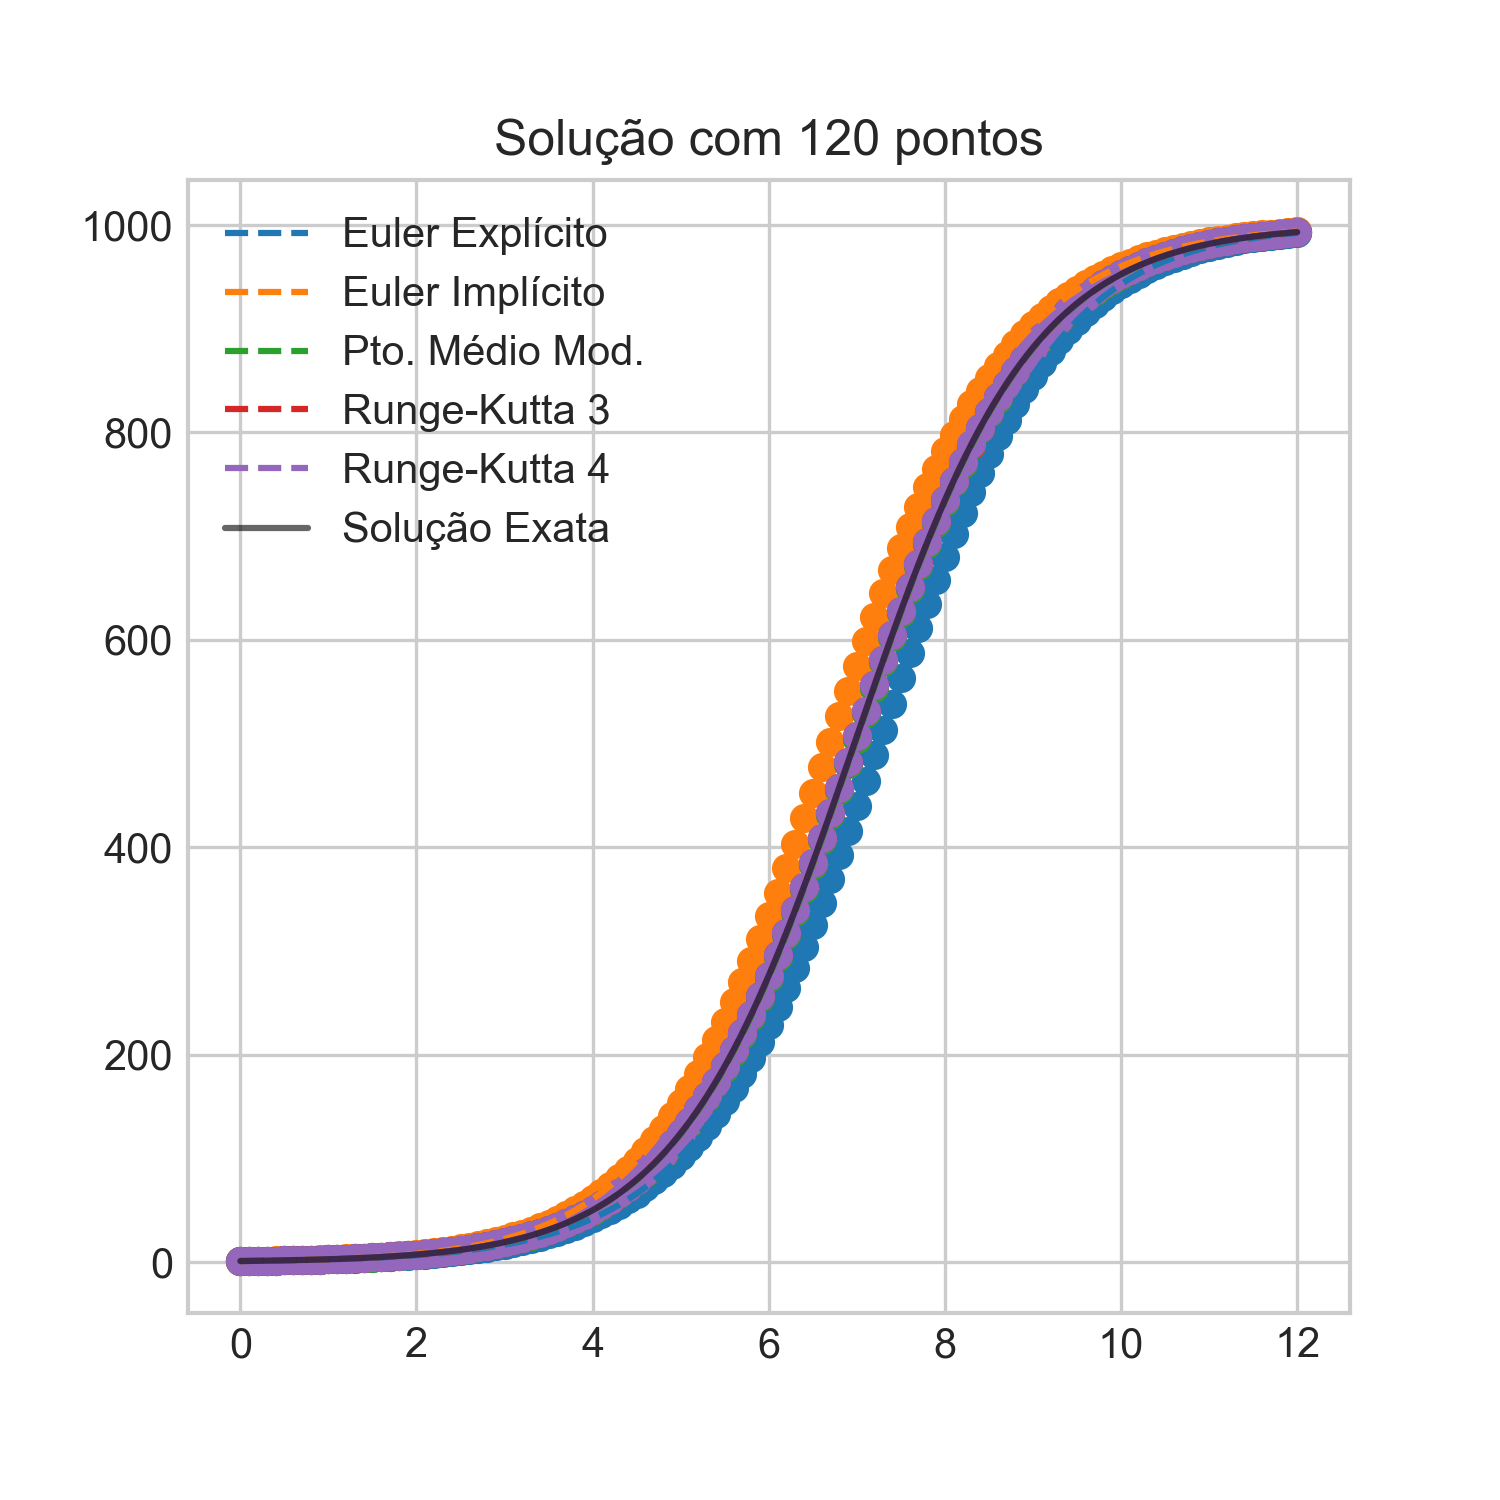
\includegraphics[height=7.8cm, width=7.8cm]{disease/solution_120.png}}
	}
	\mbox{
		\subfigure[]{
			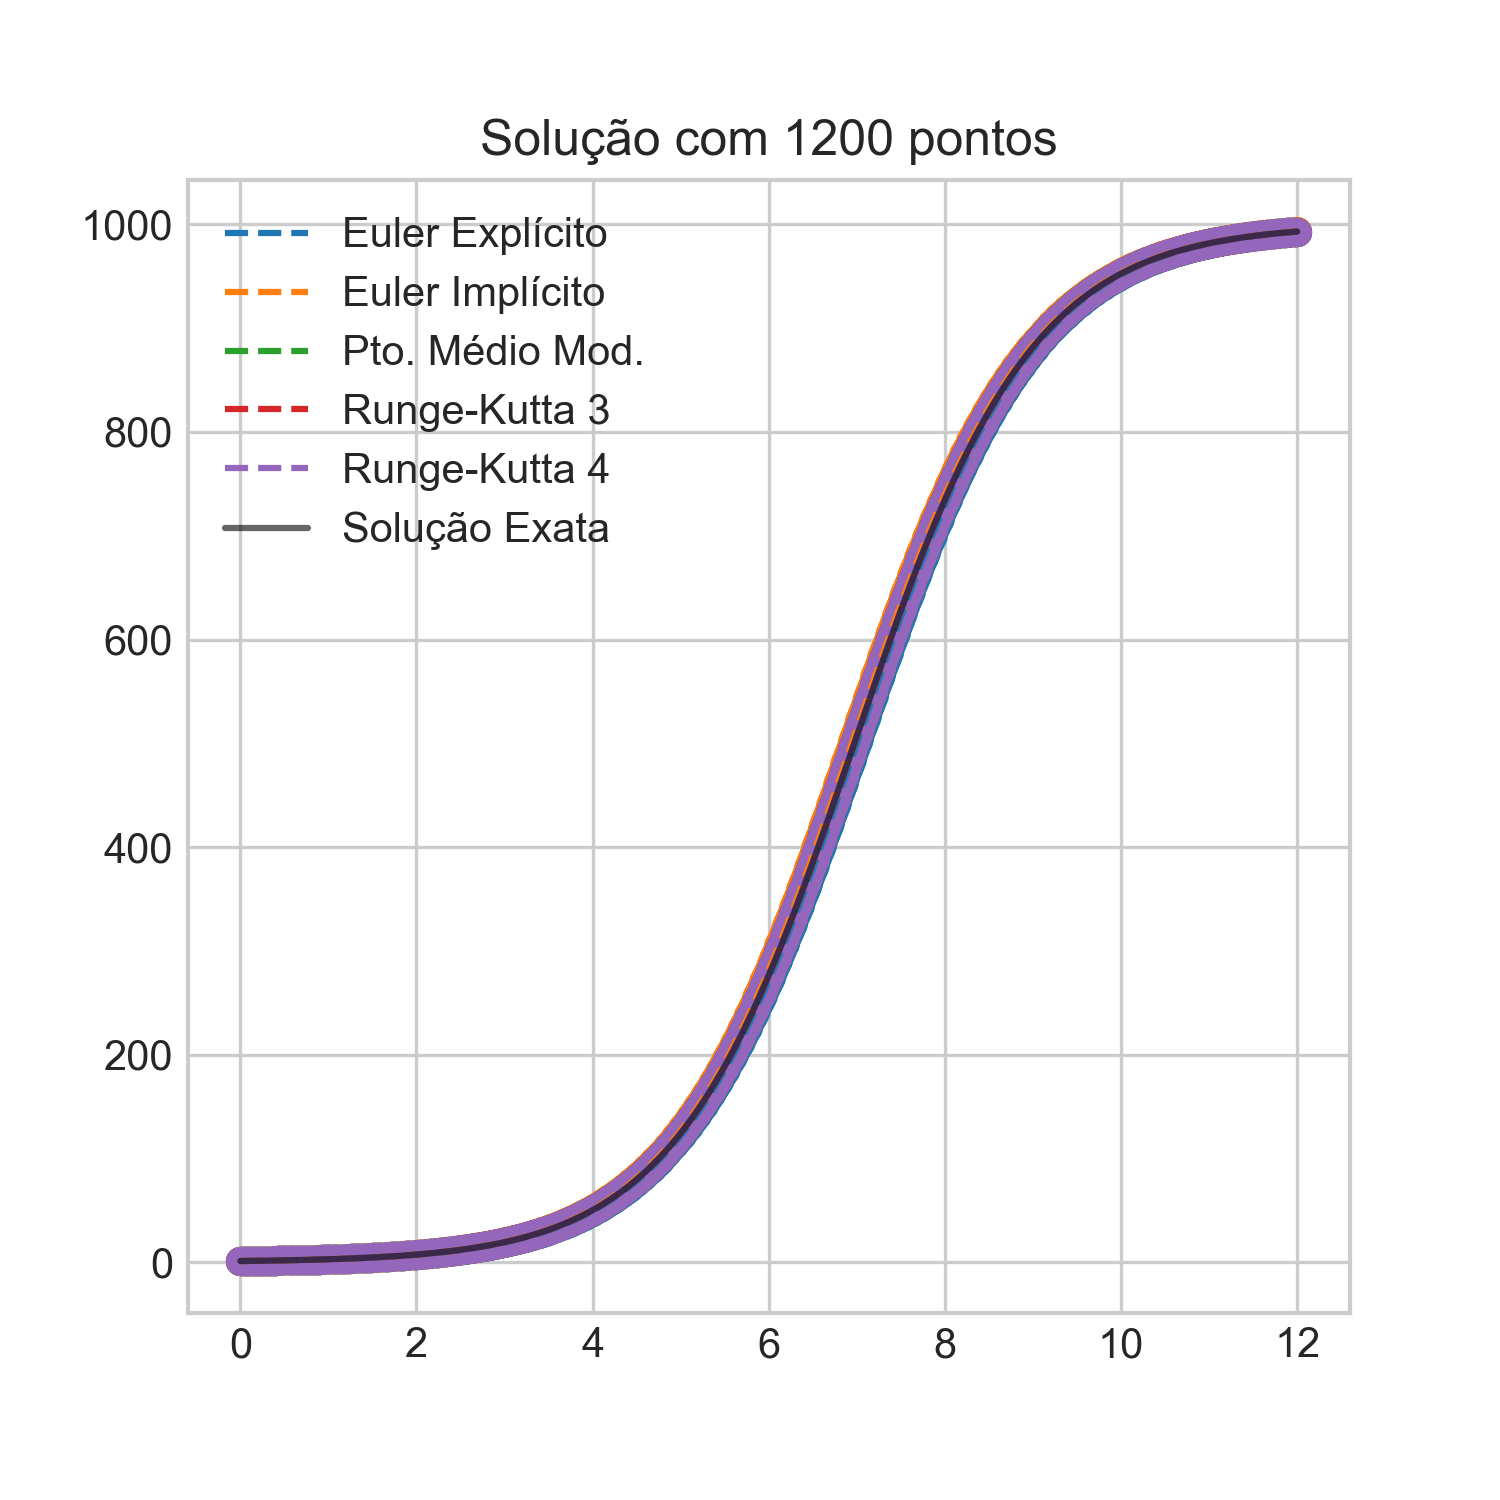
\includegraphics[height=7.8cm, width=7.8cm]{disease/solution_1200.png}}
		\subfigure[]{
			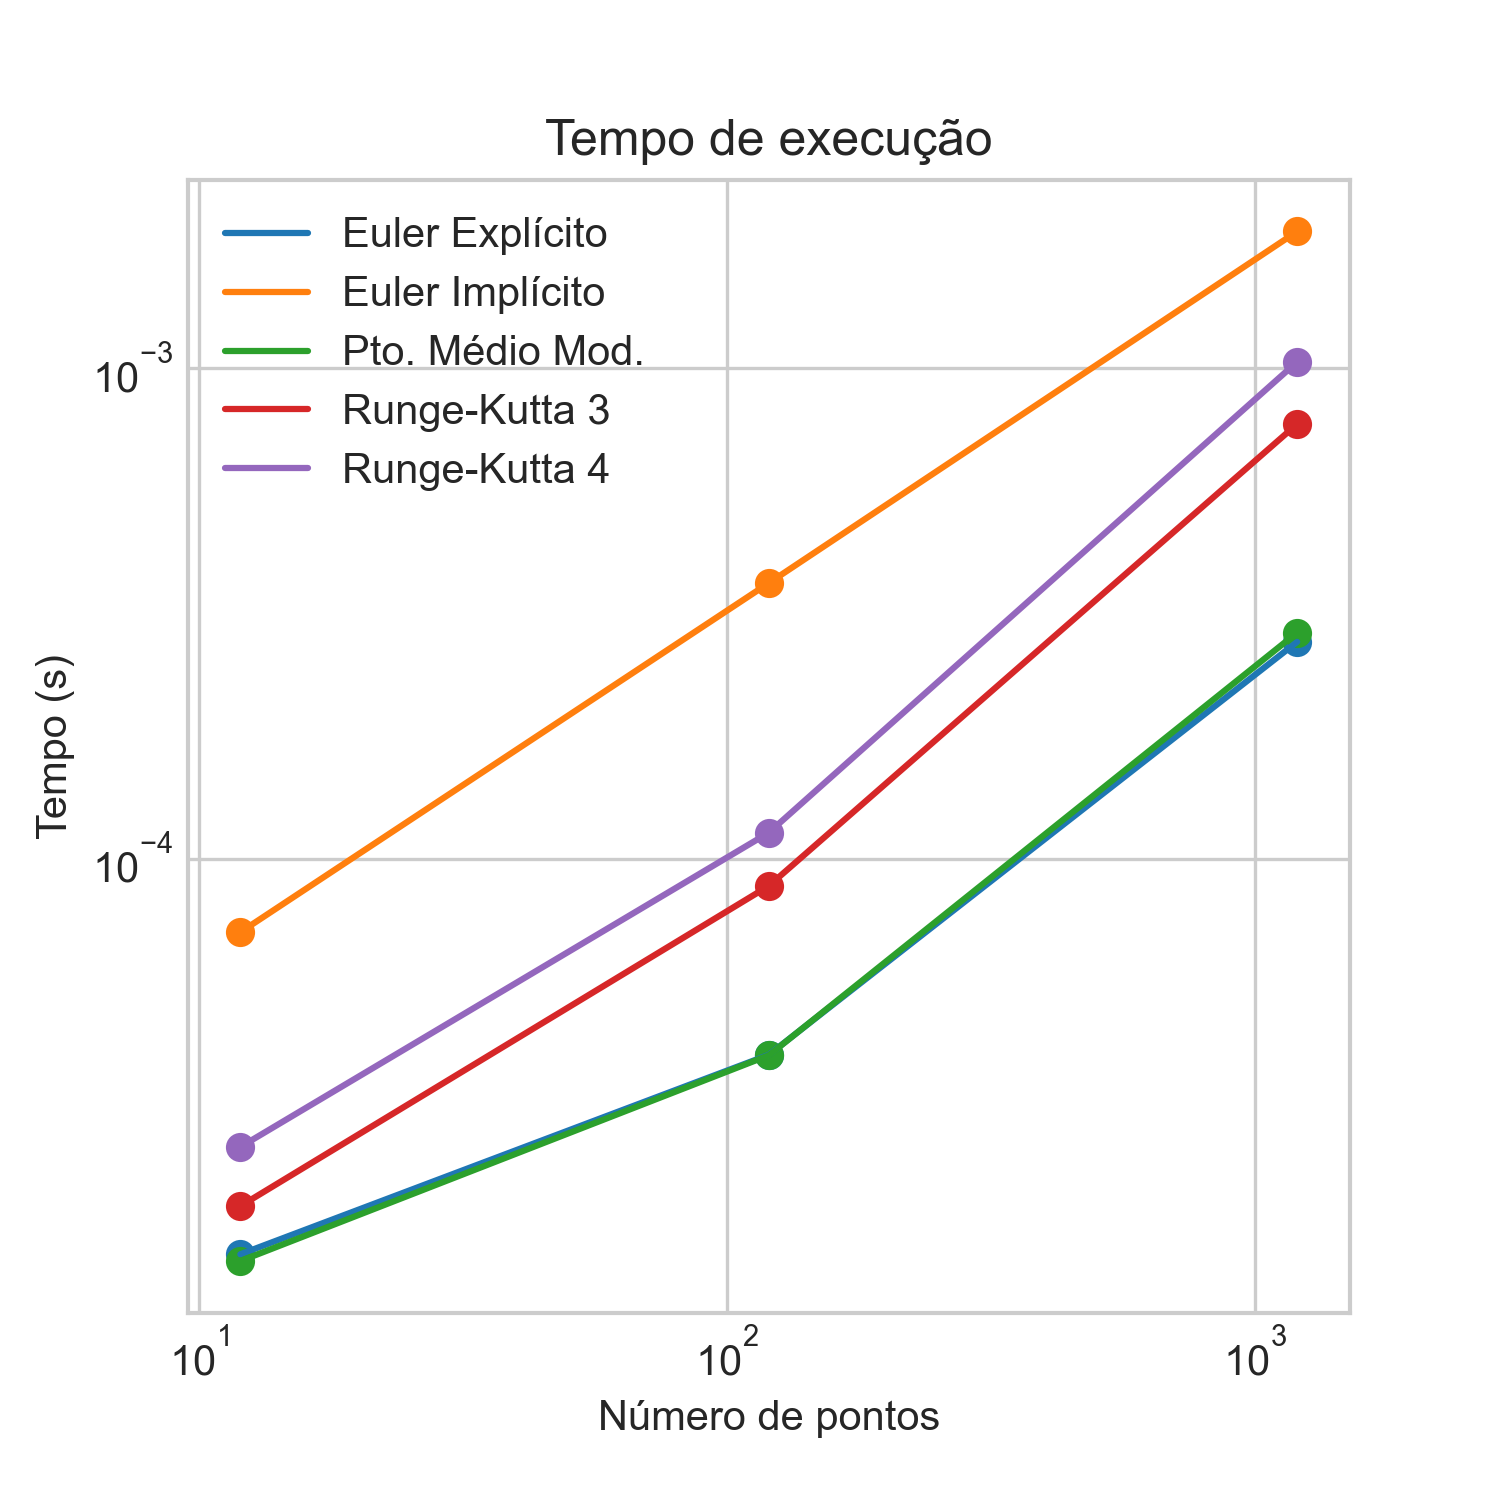
\includegraphics[height=7.8cm, width=7.8cm]{disease/timings.png}}
	}
	\caption{(a) Solução com malha grossa; (b) Solução com malha intermediária; (c) Solução com malha fina; (d) Tempos de execução de cada método. }
    \label{img:ex1_plots}
\end{figure}

Pode-se observar que à medida que o tamanho da malha diminui, as soluções se aproximam cada vez mais da solução analítica, resultando em uma redução do erro de aproximação. Além disso, o tempo de execução aumenta proporcionalmente ao número de pontos da malha.

Outra medida útil para avaliar a precisão dos métodos é o erro relativo, definido como $E_{r} = \Bigg|\dfrac{y_i - y(t_i)}{y(t_i)}\Bigg|$ para $y(t_i) \ne 0$. A Tabela \ref{tab:ex1_relative_errors} apresenta o erro relativo médio para cada método em toda a malha.

% TODO: FIX THIS (2023)
\begin{table}\label{tabela-exemplo1}
	\centering
	\begin{tabular}{|c|c|c|c|c|}
		\hline
		Ordem & \backslashbox{Método}{Pontos} & $12$                   & $120$                  & $1200$                 \\
		\hline
        \rule{0pt}{3ex} 
		1&Euler Explícito & $5.03 \times 10^{-1}$ & $8.50 \times 10^{-2}$ & $9.17 \times 10^{-3}$ \\ \rule{0pt}{3ex} 
        1&Euler Implícito & $4.06 \times 10^{+0}$ & $1.02 \times 10^{-1}$ & $9.34 \times 10^{-3}$ \\ \rule{0pt}{3ex} 
        2&Ponto Médio Modificado & $2.57 \times 10^{-1}$ & $4.08 \times 10^{-3}$ & $4.10 \times 10^{-5}$ \\ \rule{0pt}{3ex} 
        3&Runge-Kutta 3 & $3.22 \times 10^{-2}$ & $6.39 \times 10^{-5}$ & $6.85 \times 10^{-8}$ \\ \rule{0pt}{3ex} 
        4&Runge-Kutta 4 & $6.66 \times 10^{-3}$ & $1.32 \times 10^{-6}$ & $1.42 \times 10^{-10}$ \\
		\hline
		
	\end{tabular}
 \caption{Erros relativos dos métodos computacionais aplicados no PVI do Exemplo $1$.}
 \label{tab:ex1_relative_errors}
\end{table}

Nota-se novamente que métodos de maior ordem tendem a convergir mais rapidamente do que os de menor ordem. Além disso, ao reduzir o espaçamento da malha, diminui-se também o erro relativo médio. Por exemplo, ao diminuir o tamanho da malha em uma magnitude de $10^1$, reduziu-se aproximadamente $10^4$ no erro médio do método de Runge-Kutta de quarta ordem. Na Tabela \ref{tab:ex1_effective_order}, pode-se analisar a ordem efetiva de cada método utilizando (\ref{effective_order}).

\begin{table}[H]
    \centering
    \begin{tabular}{|c|c|}
        \hline
        Método & Ordem de acurácia efetiva\\
        \hline \rule{0pt}{2.5ex} 
         Euler Explícito & $1.01812$\\\rule{0pt}{2.5ex} 
         Euler Implícito & $0.98333$\\\rule{0pt}{2.5ex} 
         Ponto Médio Modificado & $2.00104$\\\rule{0pt}{2.5ex} 
         Runge-Kutta 3 & $2.87502$\\\rule{0pt}{2.5ex} 
         Runge-Kutta 4 & $3.99328$\\
         \hline
    \end{tabular}
    \caption{Ordem efetiva dos erros para cada método estudado.}
    \label{tab:ex1_effective_order}
\end{table}



\subsection{Segundo problema: capacidade de carga}\label{problem-2} \quad
O segundo problema são os estudos de Lotka-Volterra sobre a Lei de Crescimento de Populações, que exploram a capacidade de carga de um meio utilizando funções logísticas. O objetivo é determinar o tamanho máximo da população de uma espécie dada a capacidade máxima do ambiente em que vive e outros fatores, como a taxa de crescimento natural e o número atual de indivíduos vivos. Busca-se assim, simular a evolução do número de indivíduos vivos na população utilizando os métodos iterativos.


O problema pode ser descrito matematicamente com:
\begin{equation}\label{carry_equation_to_be_solved}
	\frac{dP}{dt} = \beta \cdot P \cdot \bigg(1 - \frac{P}{K}\bigg)
\end{equation}

onde:\begin{itemize}
\item $P$ é o número de indivíduos vivos; 
\item $\beta$ é a taxa de crescimento da população;
\item $K$ é a capacidade de carga máxima do sistema;
\item $t$ é a variável de tempo, medida em anos;
\end{itemize}

As equações logísticas são conhecidas pela sua forma em S. Seja $P_0$ a população inicial do problema (\ref{carry_equation_to_be_solved}), observa-se que no início do intervalo a população crescerá lentamente, pois há poucos indivíduos para reproduzirem. A partir desse ponto, $P$ crescerá cada vez mais rapidamente até se aproximar do valor de K, momento em que o crescimento diminuirá, uma vez que $\lim_{P\to K} \big(1 - \frac{P}{K}\big) = 0$. A solução geral de um problema de Lei de Crescimento de Populações de Lotka-Volterra é descrita como:
\begin{equation*}
 P(t) = \dfrac{K}{\dfrac{K - P_0}{P_0} \cdot e^{-\beta t} + 1}
\end{equation*}

Para $\beta = 1$, $K = 1000$, $P_0 = 100$ e o intervalo $[0, 12]$, o PVI a ser resolvido é dado por:
\begin{equation}\label{pvi_carrying-capacity}
    \begin{cases}
	\dfrac{dP}{dt} = \cdot P \cdot \bigg(1 - \dfrac{P}{1000}\bigg) & \\
        P(0) = 100 & t \in [0, 12]
    \end{cases}
\end{equation}
Para este problema, a solução analítica é apresentada como:
\begin{equation*}
    P(t) = \dfrac{3000}{\dfrac{3000 - 100}{100} \cdot e^{-t} + 1} = \dfrac{3000}{29e^{-t} + 1}
\end{equation*}
Utilizando os métodos estudados, a solução numérica obitida para o problema (\ref{pvi_carrying-capacity}) é ilustrada na Figura \ref{img:carry_plots}.
\begin{figure}[H]
	\centering
	\mbox{
		\subfigure[]{
			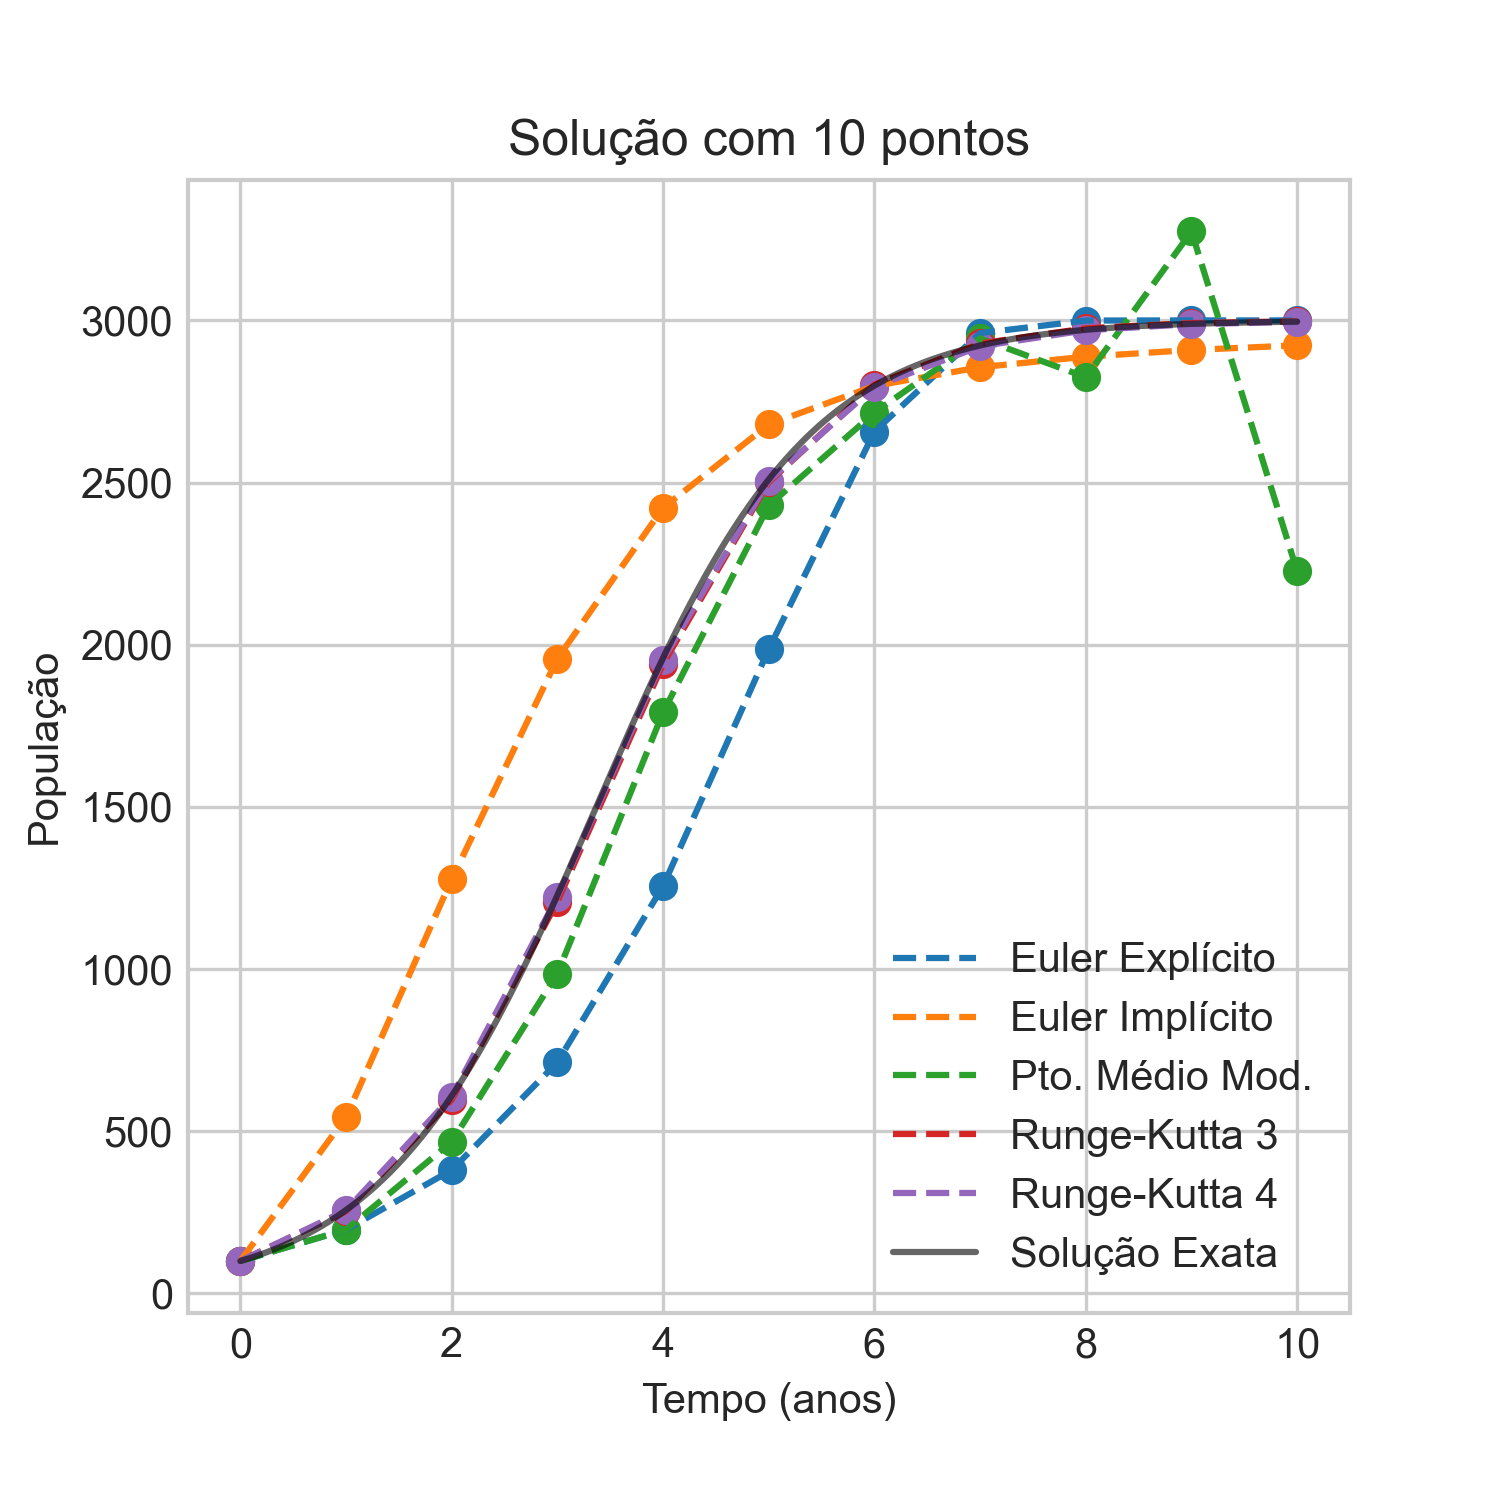
\includegraphics[height=7.8cm, width=7.8cm]{carry-capacity/carry-solution_10_300dpi.png}}
		\subfigure[]{
			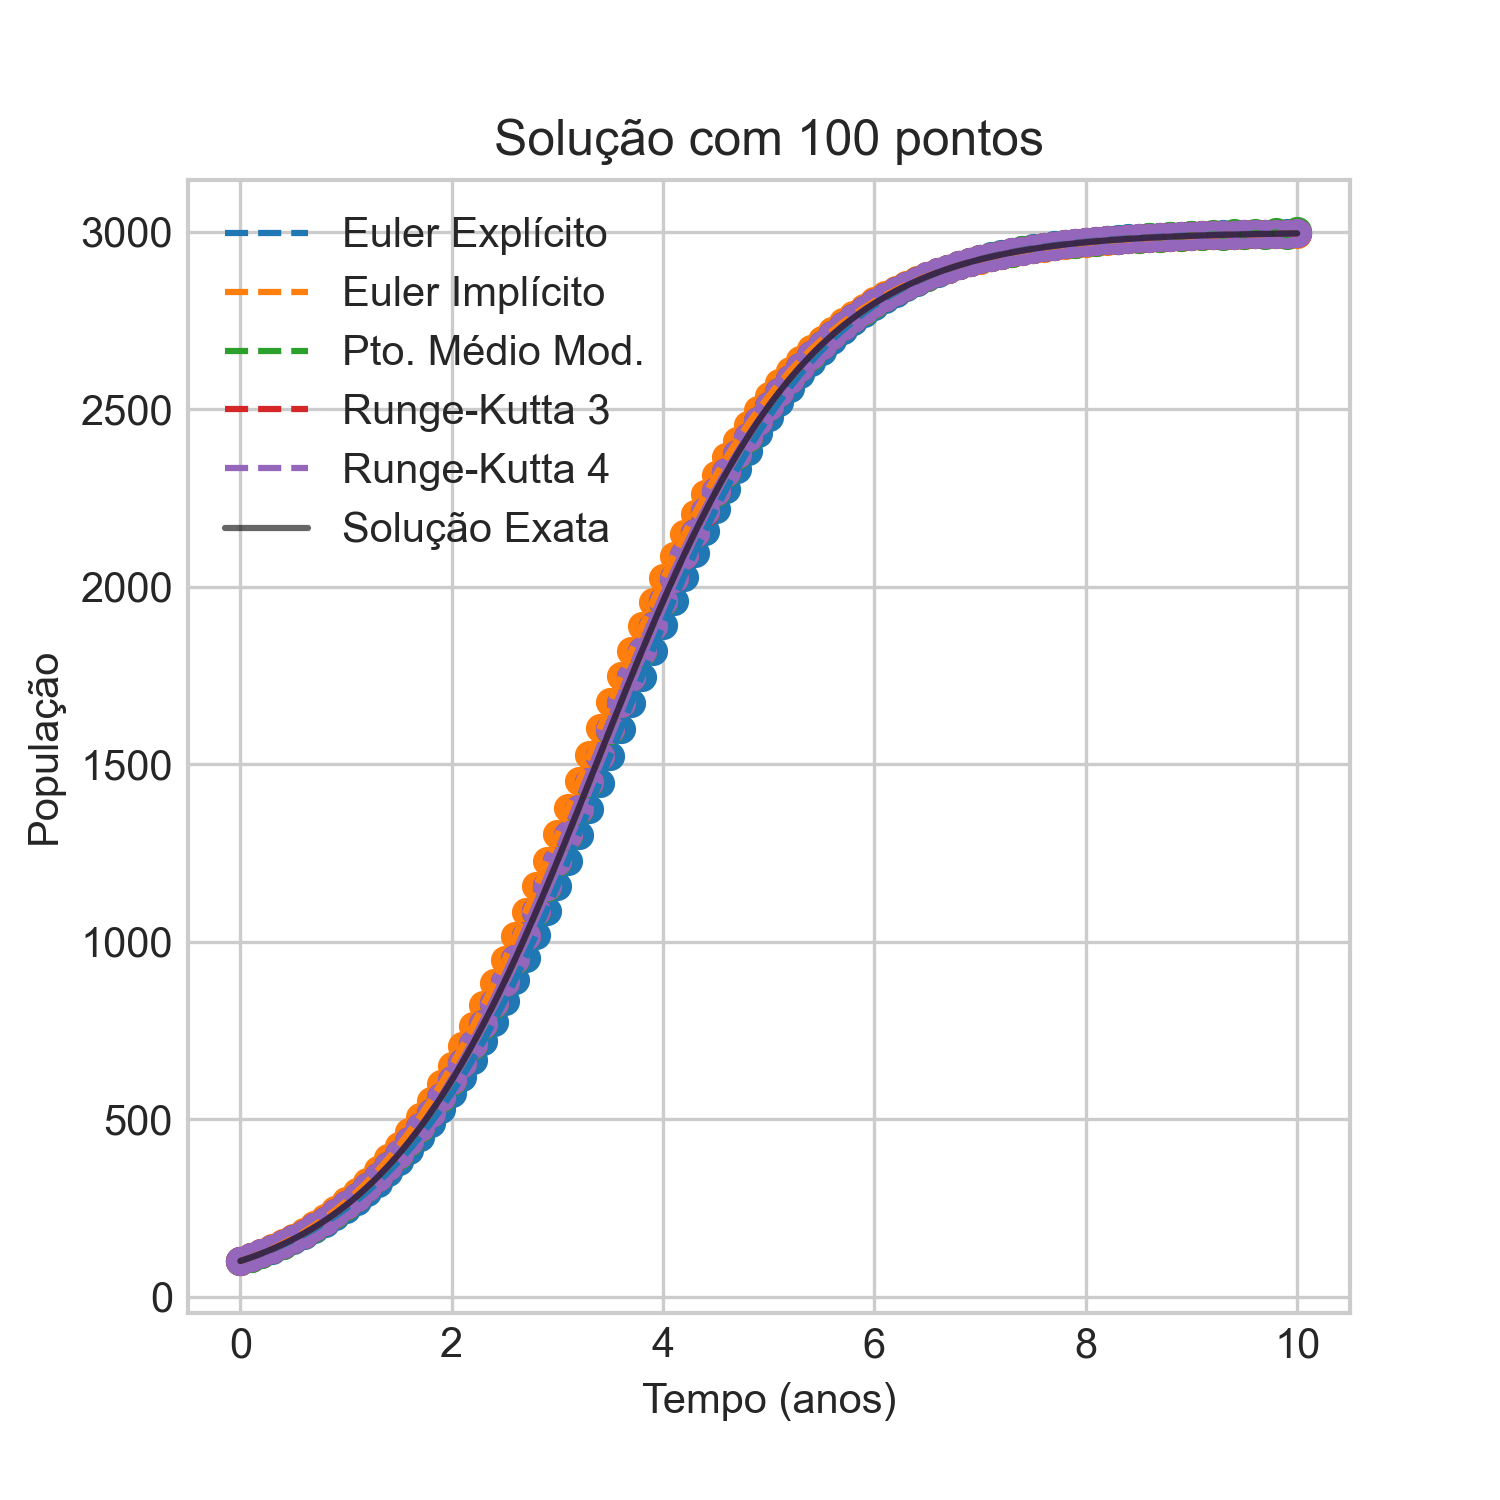
\includegraphics[height=7.8cm, width=7.8cm]{carry-capacity/carry-solution_100_300dpi.png}}
	}
	\mbox{
		\subfigure[]{
			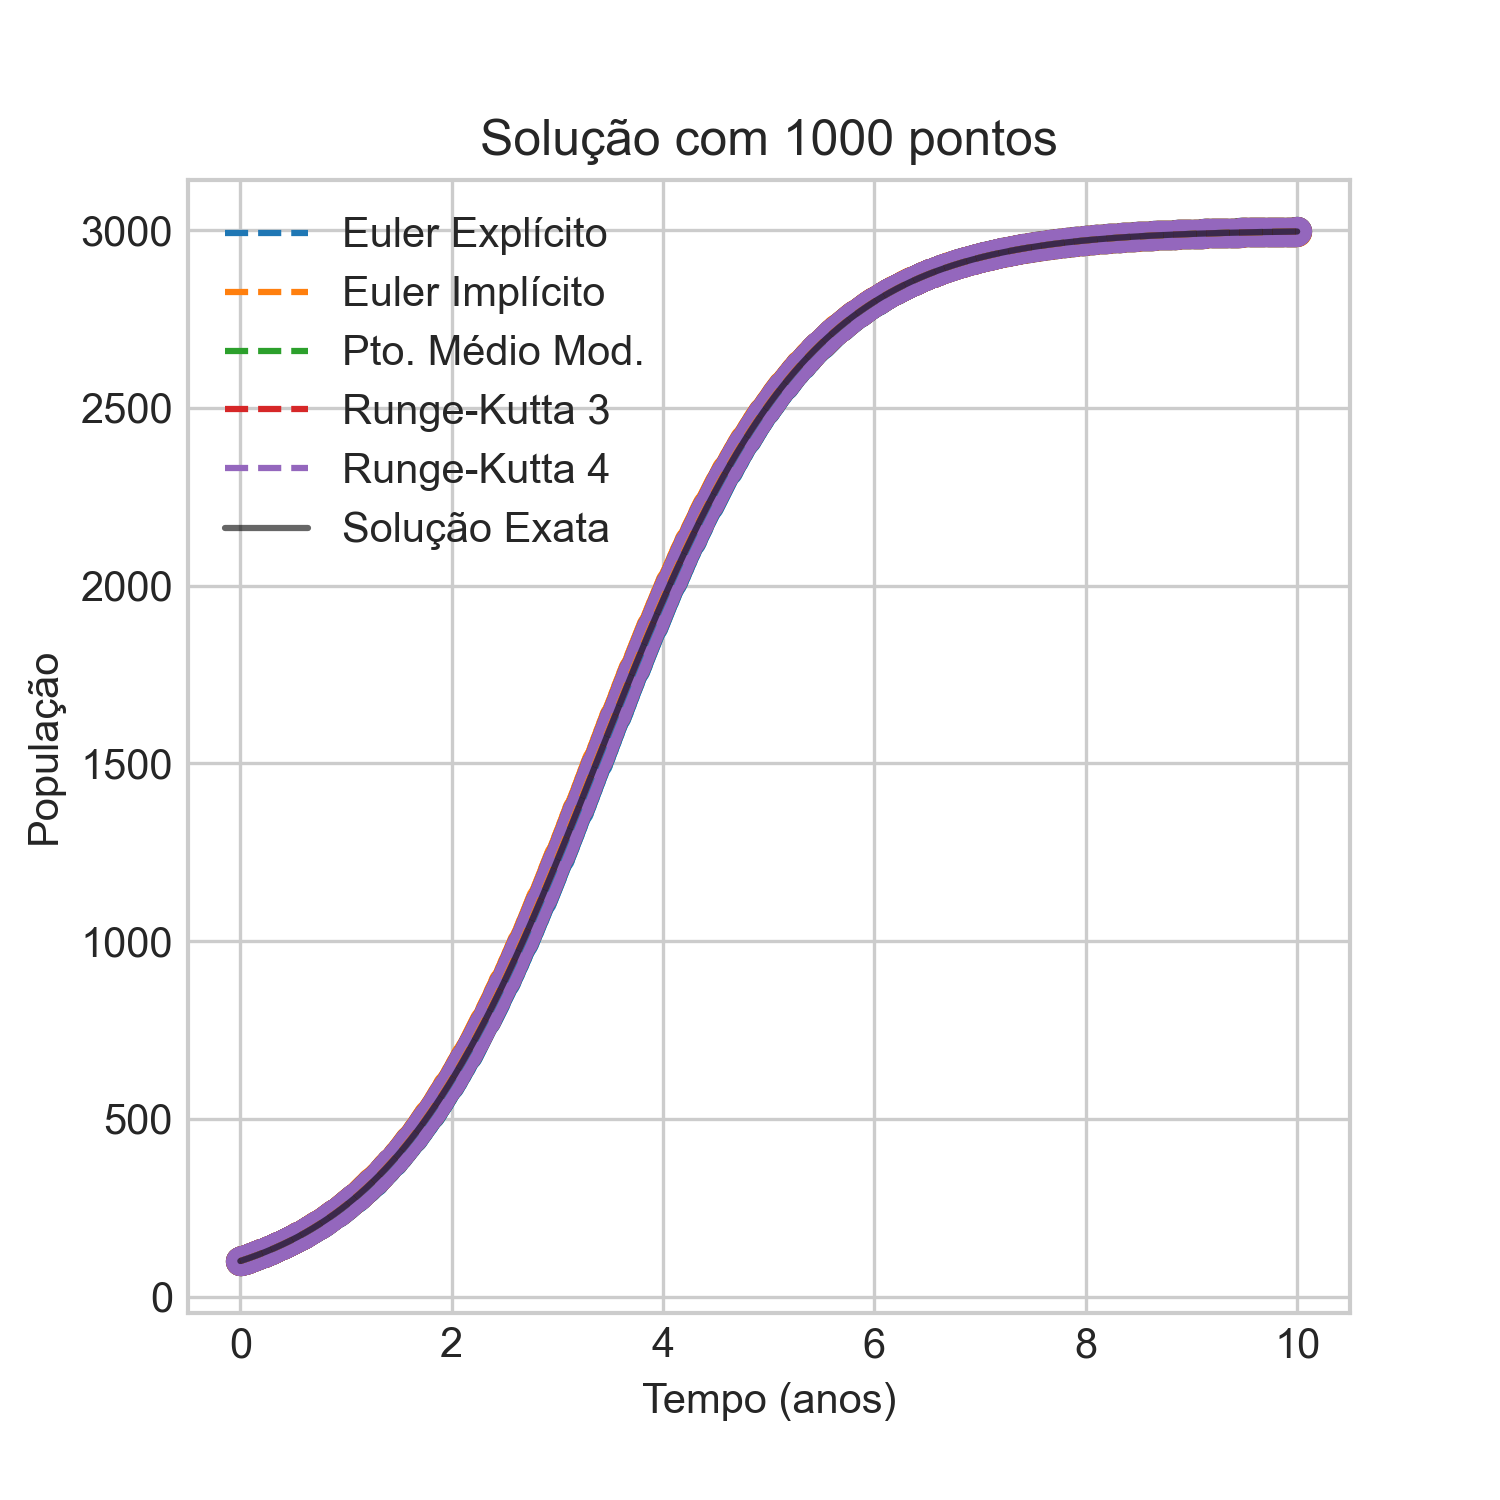
\includegraphics[height=7.8cm, width=7.8cm]{carry-capacity/carry-solution_1000_300dpi.png}}
		\subfigure[]{
			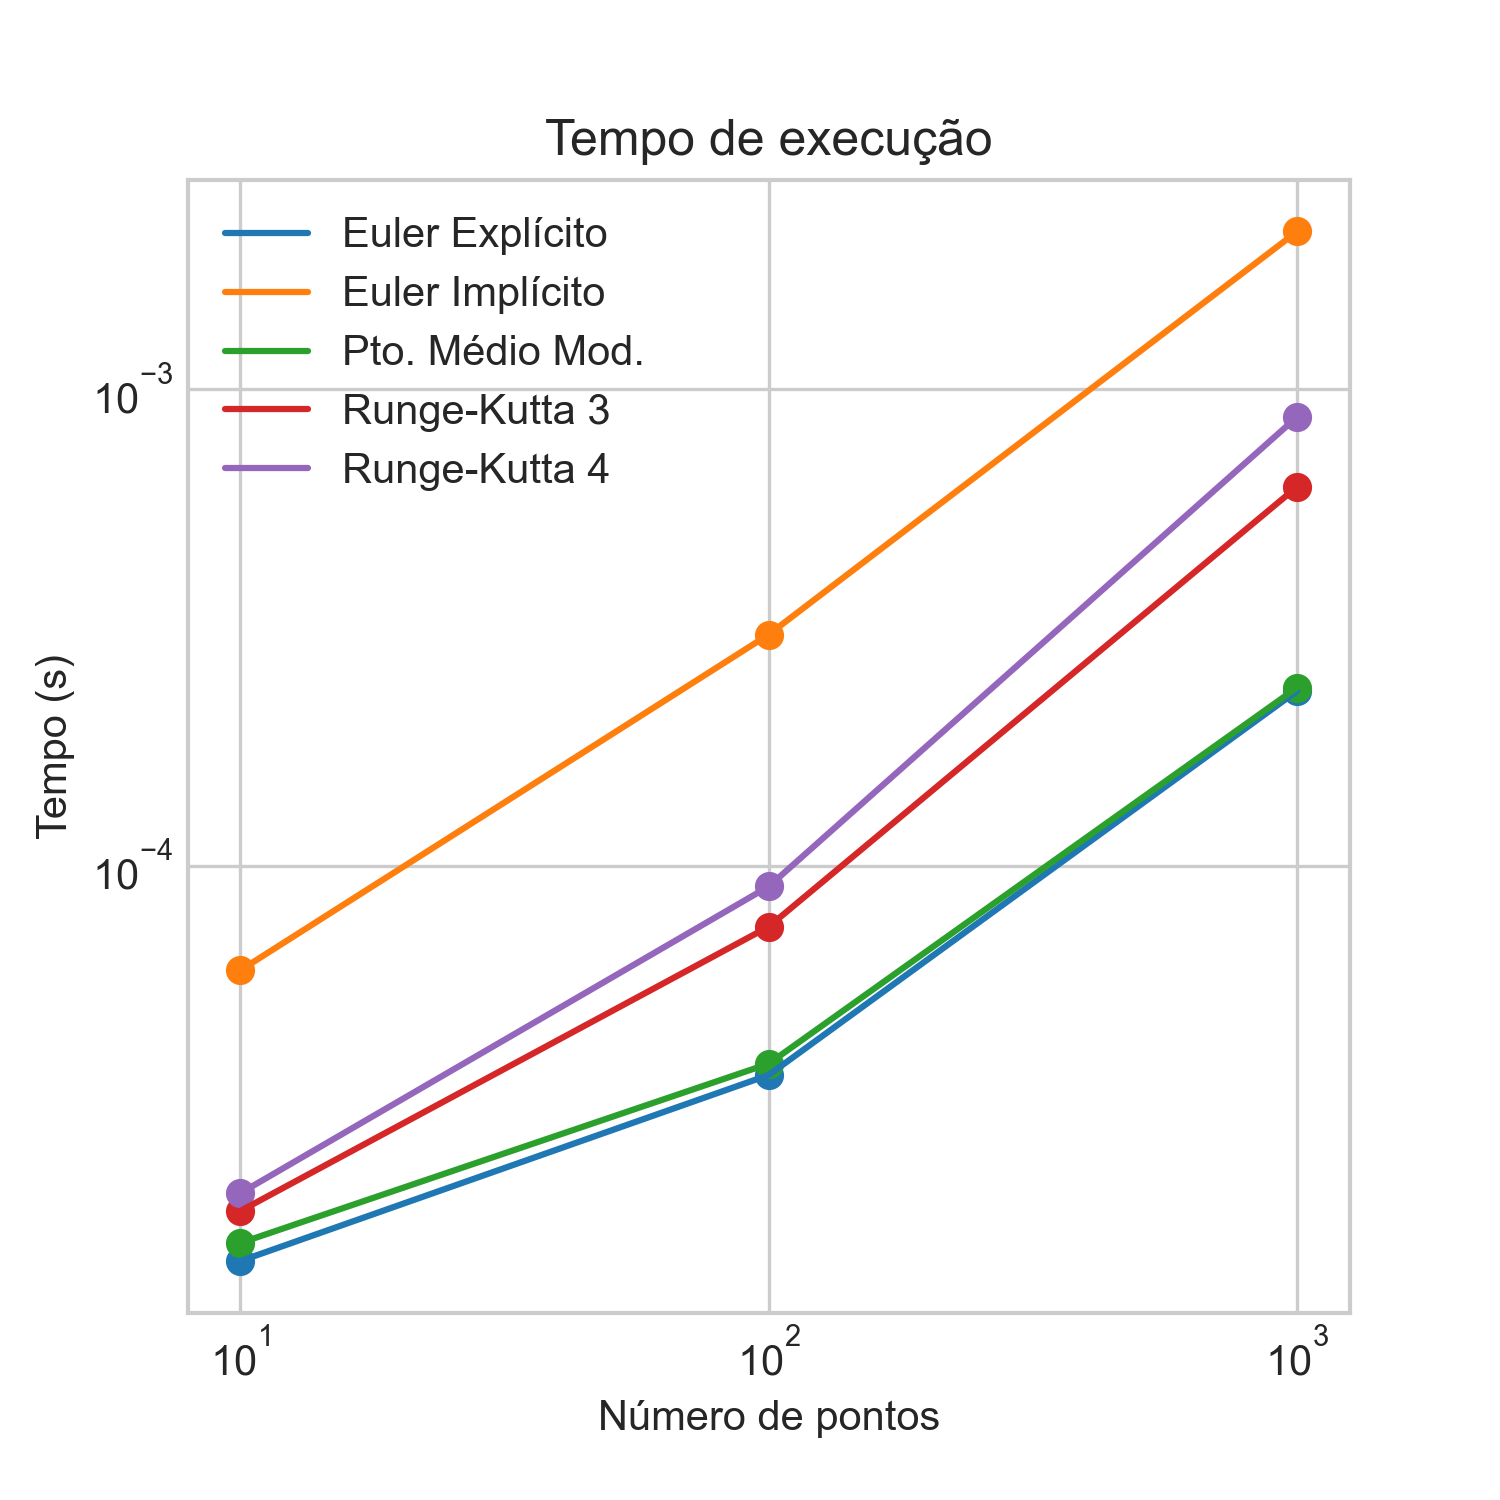
\includegraphics[height=7.8cm, width=7.8cm]{carry-capacity/timings-300dpi.png}}
	}
	\caption{(a) Solução com malha grossa; (b) Solução com malha intermediária; (c) Solução com malha fina; (d) Tempos de execução de cada método. }
    \label{img:carry_plots}
\end{figure}

Assim como no primeiro problema, ao reduzir o tamanho da malha, as soluções convergem para a solução analítica. O erro relativo médio, para cada método, está descrito na Tabela \ref{tab:carry_relative_errors}.

% TODO: Fix this (2023)
\begin{table}\label{tabela-carry}
	\centering
	\begin{tabular}{|c|c|c|c|c|}
		\hline
		Ordem & \backslashbox{Método}{Pontos} & $10$                   & $100$                  & $1000$                 \\
		\hline
        \rule{0pt}{3ex} 
		1&Euler Explícito & $1.67 \times 10^{-1}$ & $2.11 \times 10^{-2}$ & $2.17 \times 10^{-3}$ \\ \rule{0pt}{3ex}
        1&Euler Implícito & $3.19 \times 10^{-1}$ & $2.25 \times 10^{-2}$ & $2.18 \times 10^{-3}$ \\ \rule{0pt}{3ex}
        2&Ponto Médio Modificado & $9.64 \times 10^{-2}$ & $1.30 \times 10^{-3}$ & $1.31 \times 10^{-5}$ \\ \rule{0pt}{3ex}
        3&Runge-Kutta 3 & $6.65 \times 10^{-3}$ & $1.14 \times 10^{-5}$ & $1.21 \times 10^{-8}$ \\ \rule{0pt}{3ex}
        4&Runge-Kutta 4 & $1.76 \times 10^{-3}$ & $2.89 \times 10^{-7}$ & $3.05 \times 10^{-11}$ \\
		\hline
		
	\end{tabular}
 \caption{Erros relativos dos métodos computacionais aplicados no PVI do Exemplo $1$.}
 \label{tab:carry_relative_errors}
\end{table}

Observa-se novamente que os métodos de maior ordem tendem a convergir mais rapidamente do que os métodos de menor ordem. Além disso, ao diminuir o espaçamento da malha, foi possível reduzir o erro relativo médio: por exemplo, ao reduzir o tamanho da malha em uma ordem de magnitude ($10^1$), obteve-se uma redução no erro médio de cada método na ordem de $10^{O(h)}$. Vale ressaltar que a ordem efetiva de cada método pode ser analisada na Tabela \ref{tab:carry_effective_order}, utilizando a equação (\ref{effective_order}).

\begin{table}[H]
    \centering
    \begin{tabular}{|c|c|}
        \hline
        Método & Ordem de acurácia efetiva\\
        \hline \rule{0pt}{2.5ex} 
        Euler Explícito & 0.99593\\\rule{0pt}{2.5ex} 
        Euler Implícito & 1.00228\\\rule{0pt}{2.5ex} 
        Ponto Médio Modificado & 1.99196\\\rule{0pt}{2.5ex} 
        Runge-Kutta 3 & 3.04741\\\rule{0pt}{2.5ex} 
        Runge-Kutta 4 & 4.01748\\
         \hline
    \end{tabular}
    \caption{Ordem efetiva dos erros para cada método estudado.}
    \label{tab:carry_effective_order}
\end{table}

Por fim, embora a estabilidade dos métodos utilizados não tenha sido abordada neste trabalho, vale ressaltar que em ambos os exemplos o método do Ponto Médio Modificado (uma adaptação das diferenças centradas) apresentou instabilidade em sua solução, sendo mais evidente em malhas mais grossas. Embora o método do Ponto Médio Modificado seja de ordem superior ao método de Euler Explícito, mantendo um custo computacional semelhante, como pode ser visto nas Figuras $\ref{img:ex1_plots}d$ e $\ref{img:carry_plots}d$, está mais sujeito a instabilidade numérica e requer condições mais restritas de espaçamento de malha \cite{ascher2008numerical}.

%%%%%%%%%%%%%%%%%%%%%%%%%%%%%%%%%%%%%%%%%%%%%%%%
\subsection{Terceiro problema: populações de predadores e presas}\label{problem-3} \quad
O terceiro problema consiste em uma equação competitiva de Lotka-Volterra \cite{goel1971} que modela a dinâmica de populações de predadores e presas. Esse modelo considera duas populações, uma de predadores $A$ e outra de presas $B$, tal que:

\emph{
	No início de um período, as presas se reproduzem e, ao final do período, cada indivíduo em média produz $r$ filhos. As presas não morrem naturalmente, mas estão sujeitas a serem predadas com uma probabilidade $p$. Por outro lado, os predadores morrem rapidamente de fome e, se não são alimentados, morrem na proporção $s$. A taxa de reprodução dos predadores está relacionada à sua capacidade de alimentação, que depende da quantidade de presas vivas.}". Adaptado de \cite{burkardt2009}.

O problema em questão é descrito matematicamente por um sistema de equações diferenciais ordinárias, dado por:

\begin{equation*}\label{predator_formula}
	\dfrac{dA}{dt} = r_AAB - sA
\end{equation*}

\begin{equation*}\label{prey_formula}
	\dfrac{dB}{dt} = r_BB - pAB
\end{equation*}

onde:

\begin{itemize}
\item $A$ é o número de predadores vivos;
\item $B$ é o número de presas vivas;
\item $r_A$ é a taxa de crescimento da população de predadores;
\item $r_B$ é a taxa de crescimento da população de presas;
\item $p$ é a probabilidade de uma presa ser capturada e morta por um predador;
\item $s$ é a proporção de predadores que morrem de fome;
\item $t$ é a variável temporal, medida em anos.
\end{itemize}

Considerando as populações iniciais $A_0 = 100$ e $B_0 = 4000$, e os valores dos parâmetros $r_A = 3 \times 10^{-3}$, $r_B = 3$, $p = 1 \times 10^{-2}$ e $s = 10$, obtêm-se o seguinte problema de valor inicial (PVI):

\begin{equation}\label{pvi-predator-prey}
	\begin{cases}
		\dfrac{dA}{dt} = 0.003AB - 10A &                            \\[3mm]
        \dfrac{dB}{dt} = 3B - 0.01AB   &                            \\[2mm]
		A(0) = 100                    &                            \\
        B(0) = 4000                   & \text{ com } t \in [0, 10] 
	\end{cases}
\end{equation}

Para resolver este problema, foram aplicados os métodos de Euler Implícito e Runge-Kutta de 4ª ordem com 500 pontos, visto que ambos geram resultados representativos. Os gráficos das soluções obtidas por estes métodos estão representados nas Figuras \ref{img:explicit_euler_plots} e \ref{img:rk4_plots}.
\begin{figure}[H]
	\centering
	\mbox{
		\subfigure[]{
			\includegraphics[height=8cm, width=8cm]{predator-prey/predator_prey-300dpi-Euler_Implícito-500points-2d.png}}
		\subfigure[]{
			\includegraphics[height=8cm, width=8cm]{predator-prey/predator_prey-300dpi-Euler_Implícito-500points-2d-up.png}}
	}
	\mbox{
		\subfigure[]{
			\includegraphics[height=12cm, width=12cm]{predator-prey/predator_prey-300dpi-Euler_Implícito-500 points.png}}
	}
	\caption{Método de Euler Implícito - (a) Evolução de ambas populações temporalmente; (b) Número de indivíduos vivos simultaneamente em diferentes instantes de tempo; (c) Representação tridimensional da evolução do problema.}
    \label{img:explicit_euler_plots}
\end{figure}

\begin{figure}[H]
	\centering
	\mbox{
		\subfigure[]{
			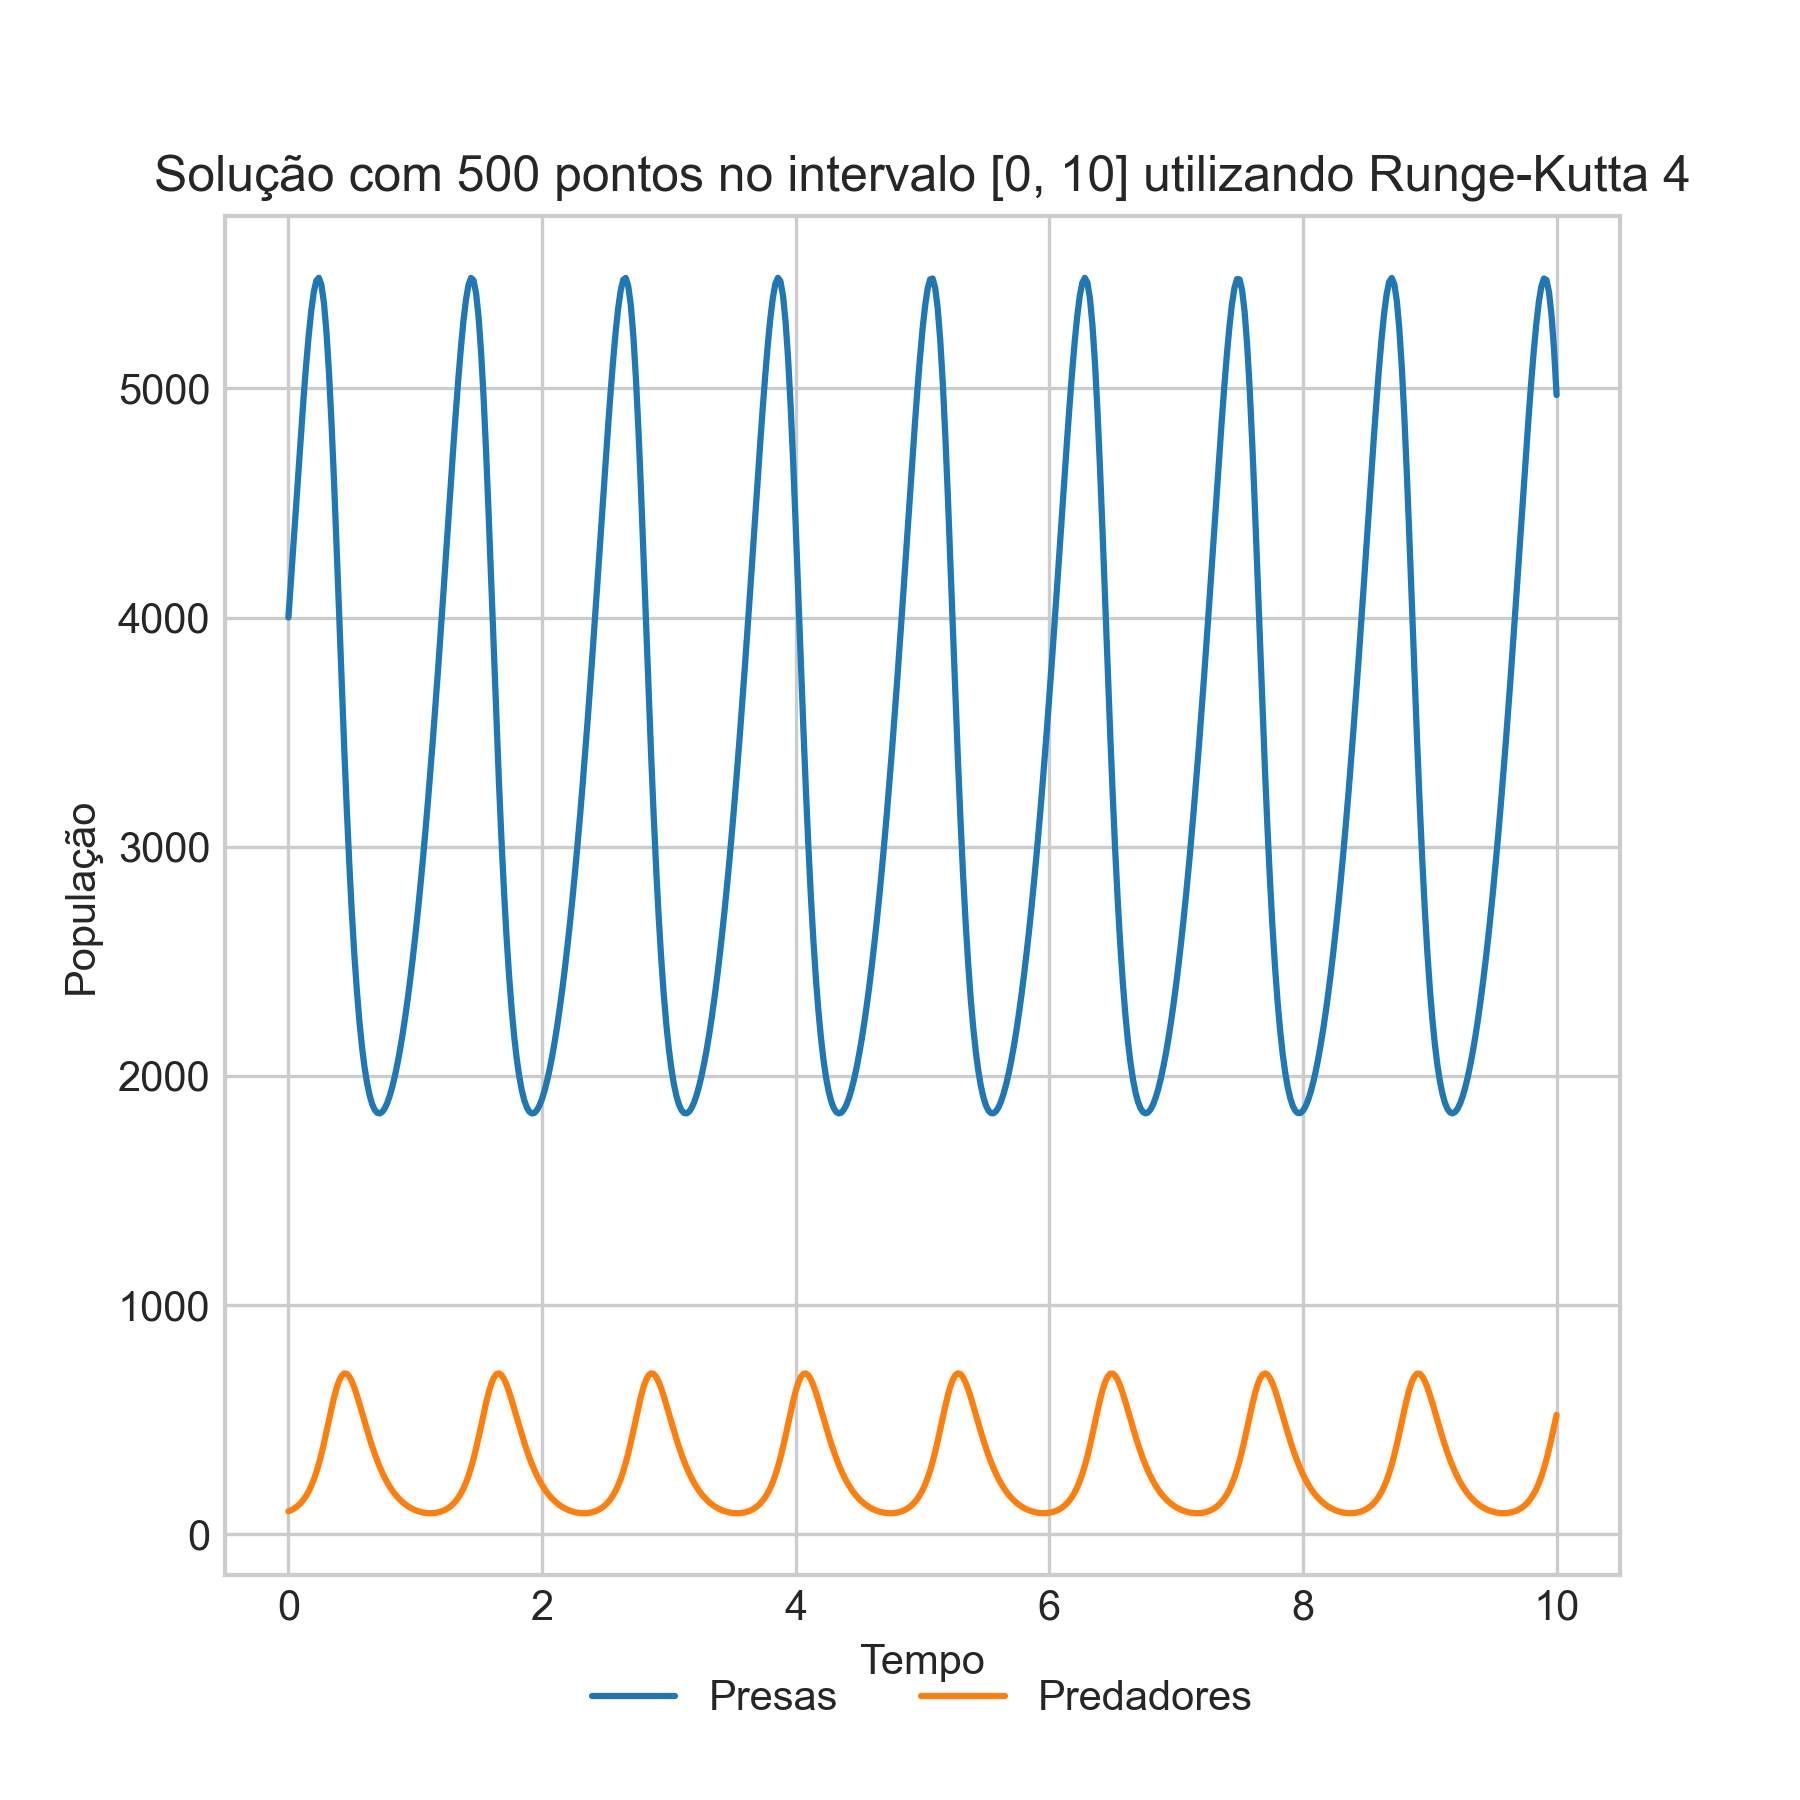
\includegraphics[height=8cm, width=8cm]{predator-prey/predator_prey-300dpi-Runge-Kutta_4-500points-2d.png}}
		\subfigure[]{
			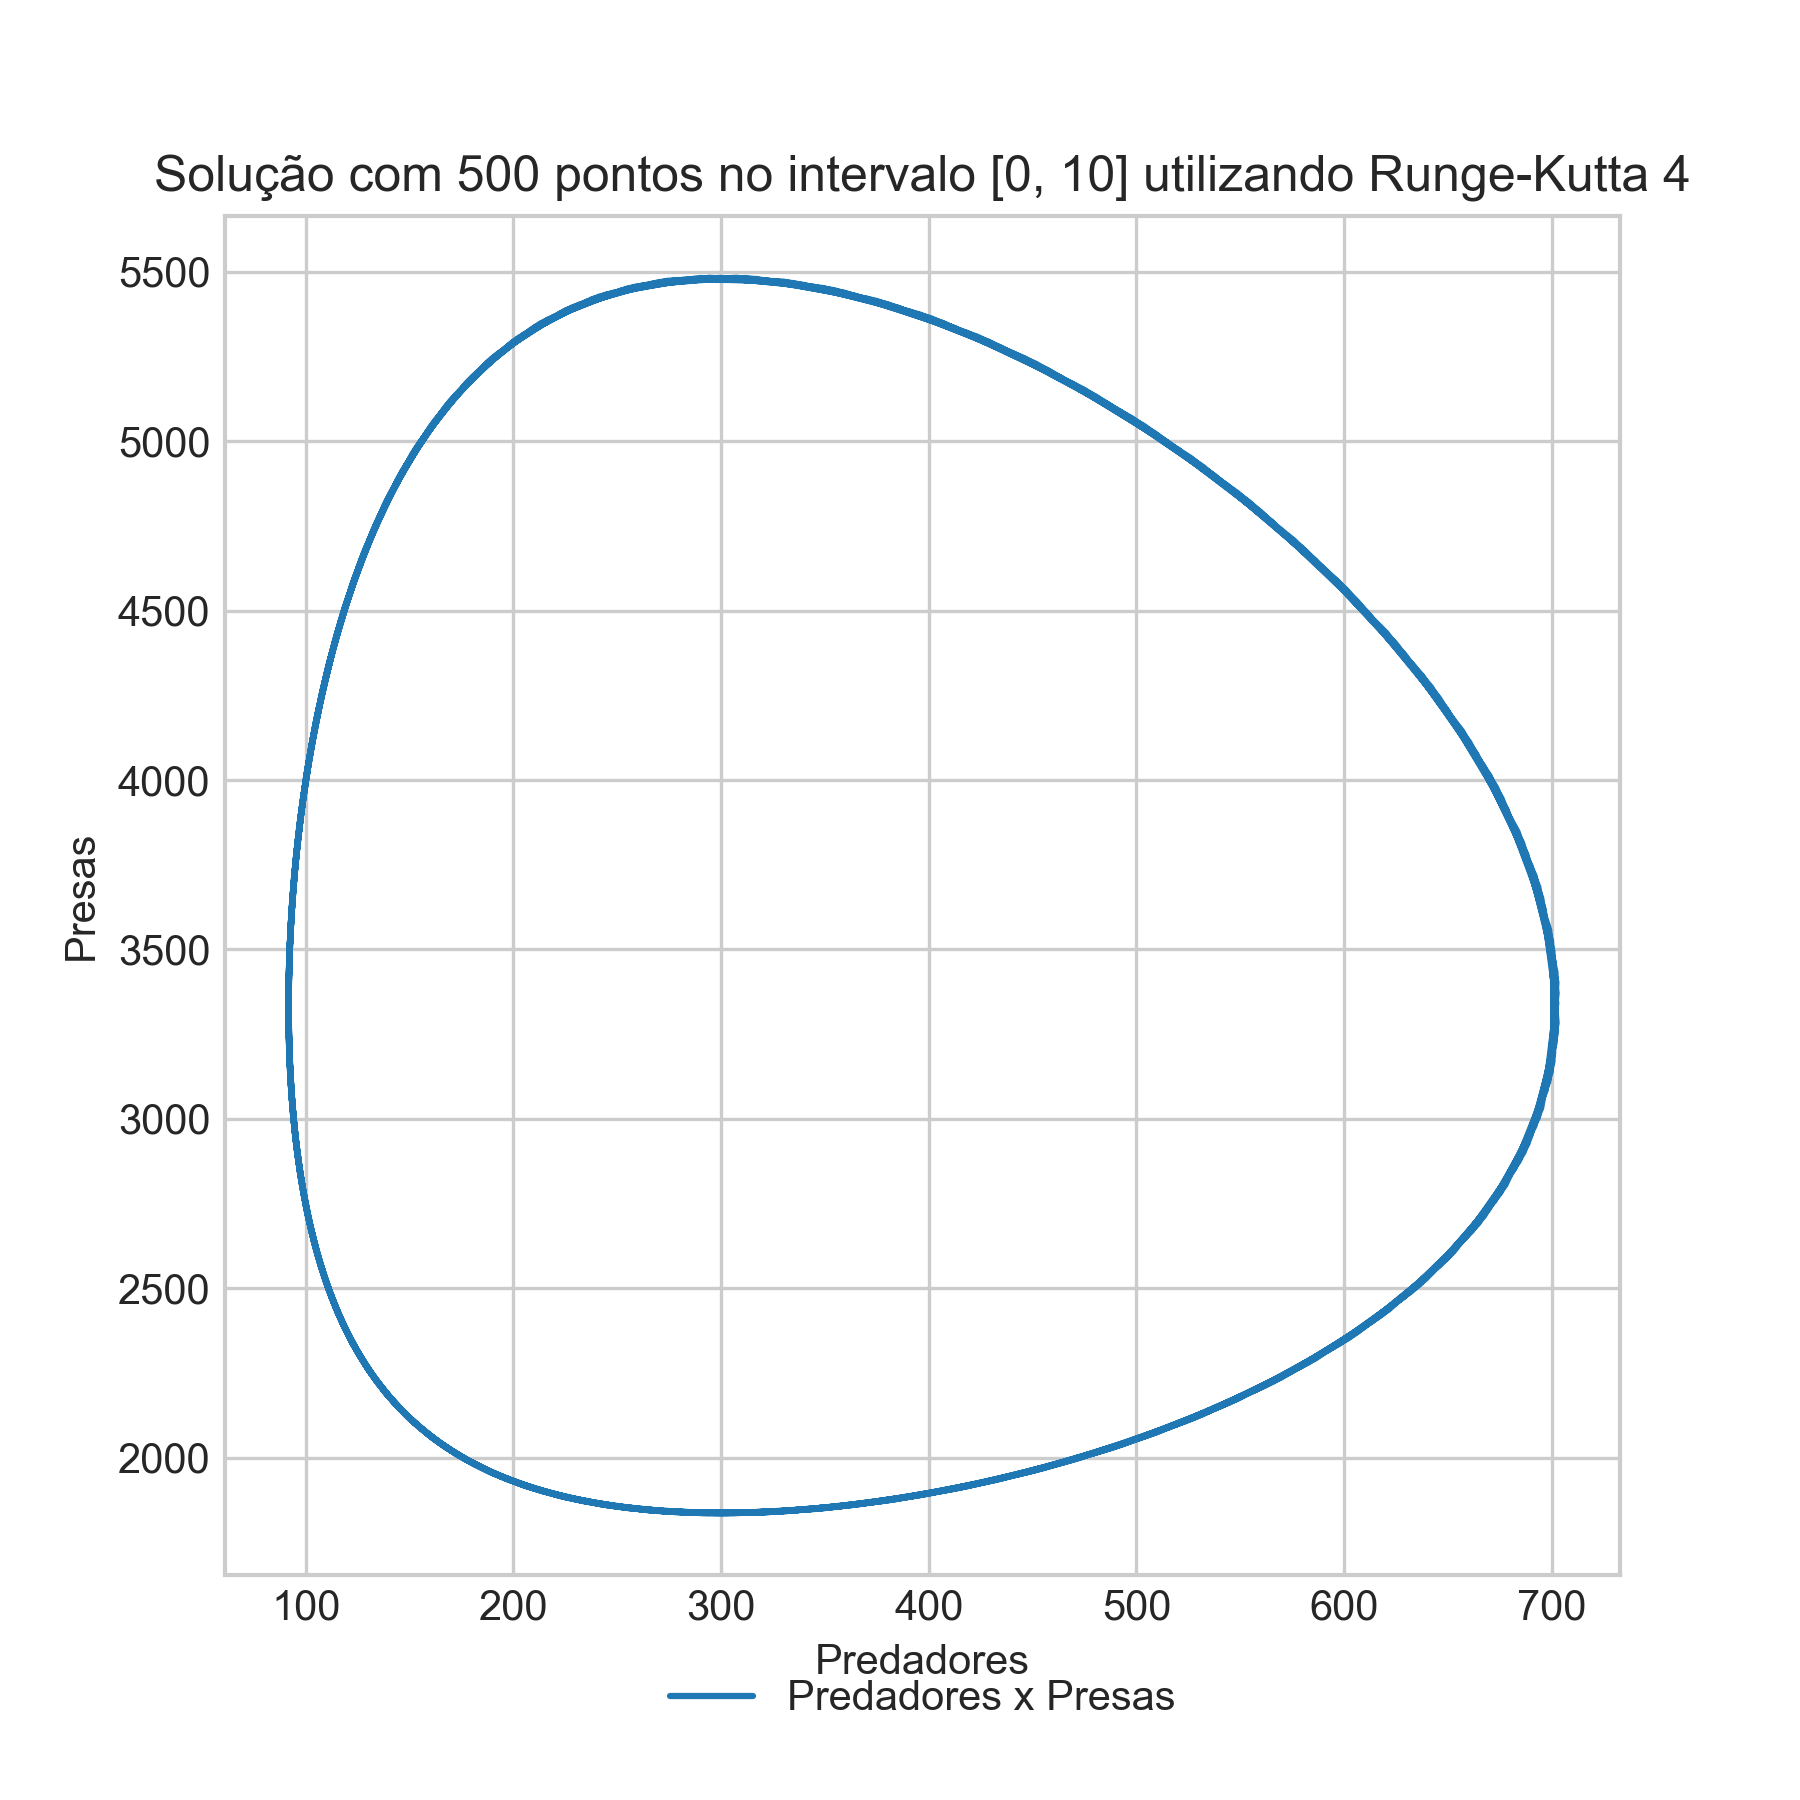
\includegraphics[height=8cm, width=8cm]{predator-prey/predator_prey-300dpi-Runge-Kutta_4-500points-2d-up.png}}
	}
	\mbox{
		\subfigure[]{
			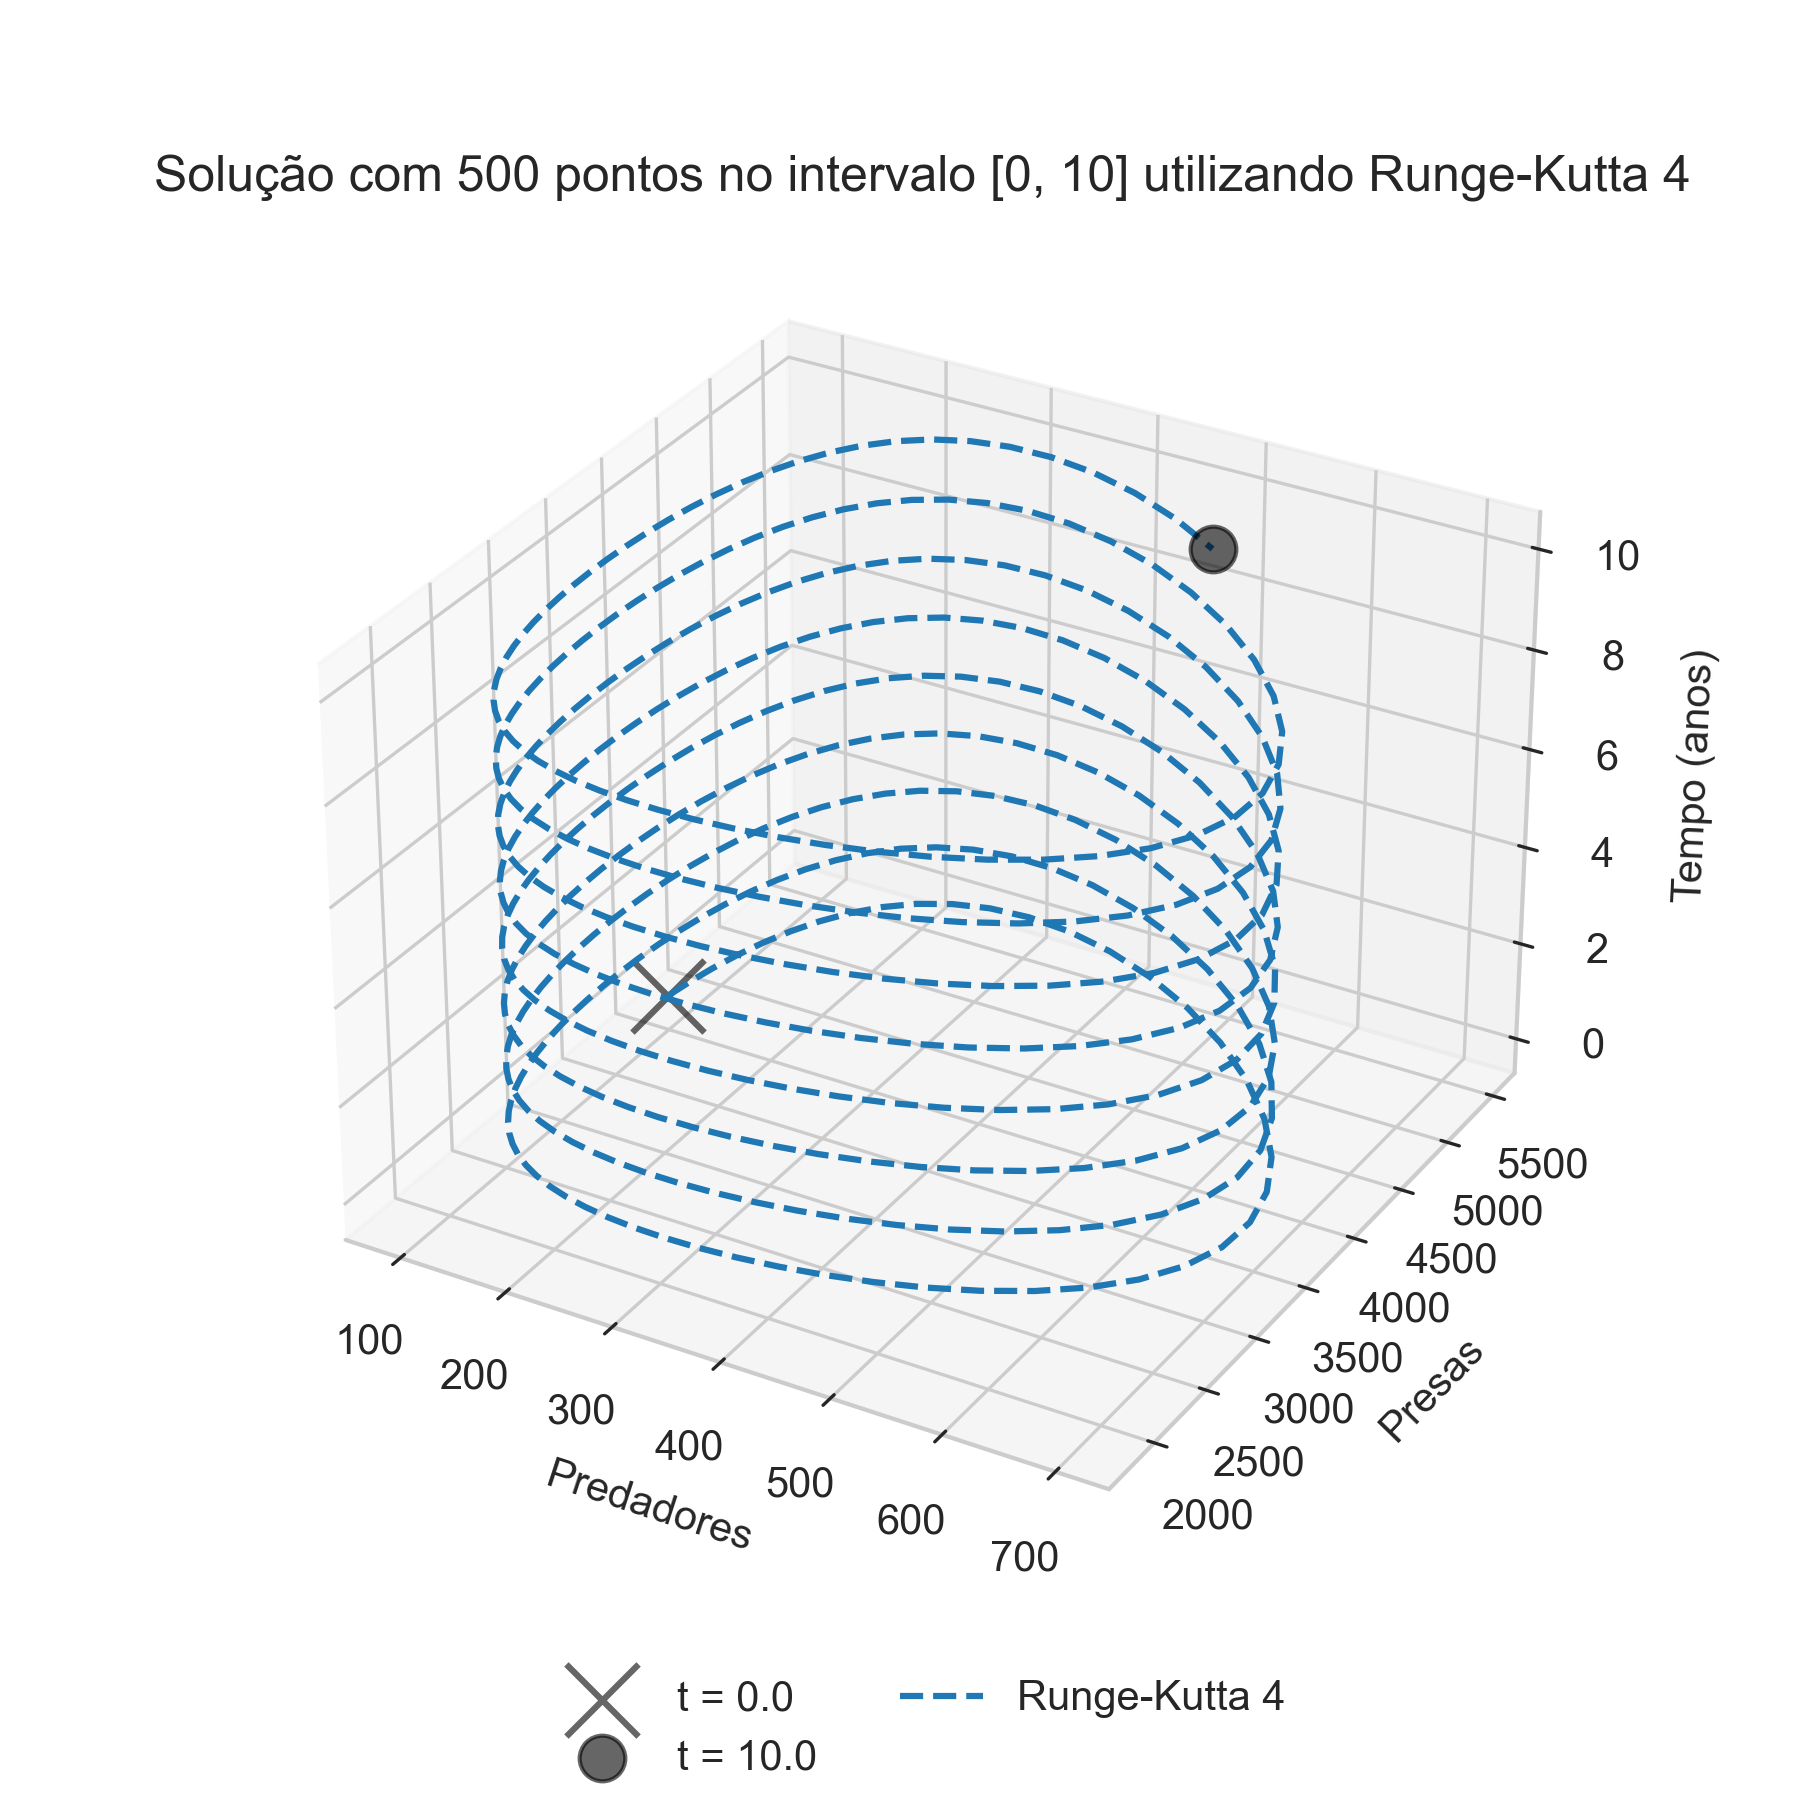
\includegraphics[height=12cm, width=12cm]{predator-prey/predator_prey-300dpi-Runge-Kutta_4-500 points.png}}
	}
	\caption{Método de Runge-Kutta de 4ª ordem - (a) Evolução de ambas populações temporalmente; (b) Número de indivíduos vivos simultaneamente em diferentes instantes de tempo; (c) Representação tridimensional da evolução do problema.}
    \label{img:rk4_plots}
\end{figure}

Constata-se que ambas soluções simulam de forma semelhante a relação de predação, onde a população de predadores cresce quando há muitas presas para se alimentar, assim como a população de presas cresce vertiginosamente quando há poucos predadores e vice-versa.

Na Figura \ref{img:explicit_euler_plots}, é possível observar que o método de Euler Implícito reduz a amplitude dos ciclos das populações ao longo do tempo, resultando em um comportamento espiral. A partir do início do intervalo, cada ano manteve o comportamento da curva, mas reduziu a variação da população. Embora novos indivíduos surjam e outros faleçam, a quantidade de indivíduos vivos simultaneamente tende a um valor constante.

Ao estudar a solução pelo método explícito de quarta ordem, observa-se que na Figura \ref{img:rk4_plots}, forma-se um gráfico periódico, em que cada ano reproduz o anterior identicamente.

Para verificar se os resultados convergem para a solução apropriada do problema, é utilizada a mesma técnica de refinamento de malha aplicada nos problemas (\ref{problem-1}) e (\ref{problem-2}). Essa técnica utiliza uma malha grossa, intermediária e fina para obter resultados cada vez mais precisos. Os resultados são ilustrados na Figura \ref{img:comparison_plots}.

\begin{figure}[H]
	\centering
	\mbox{
		\subfigure[]{
			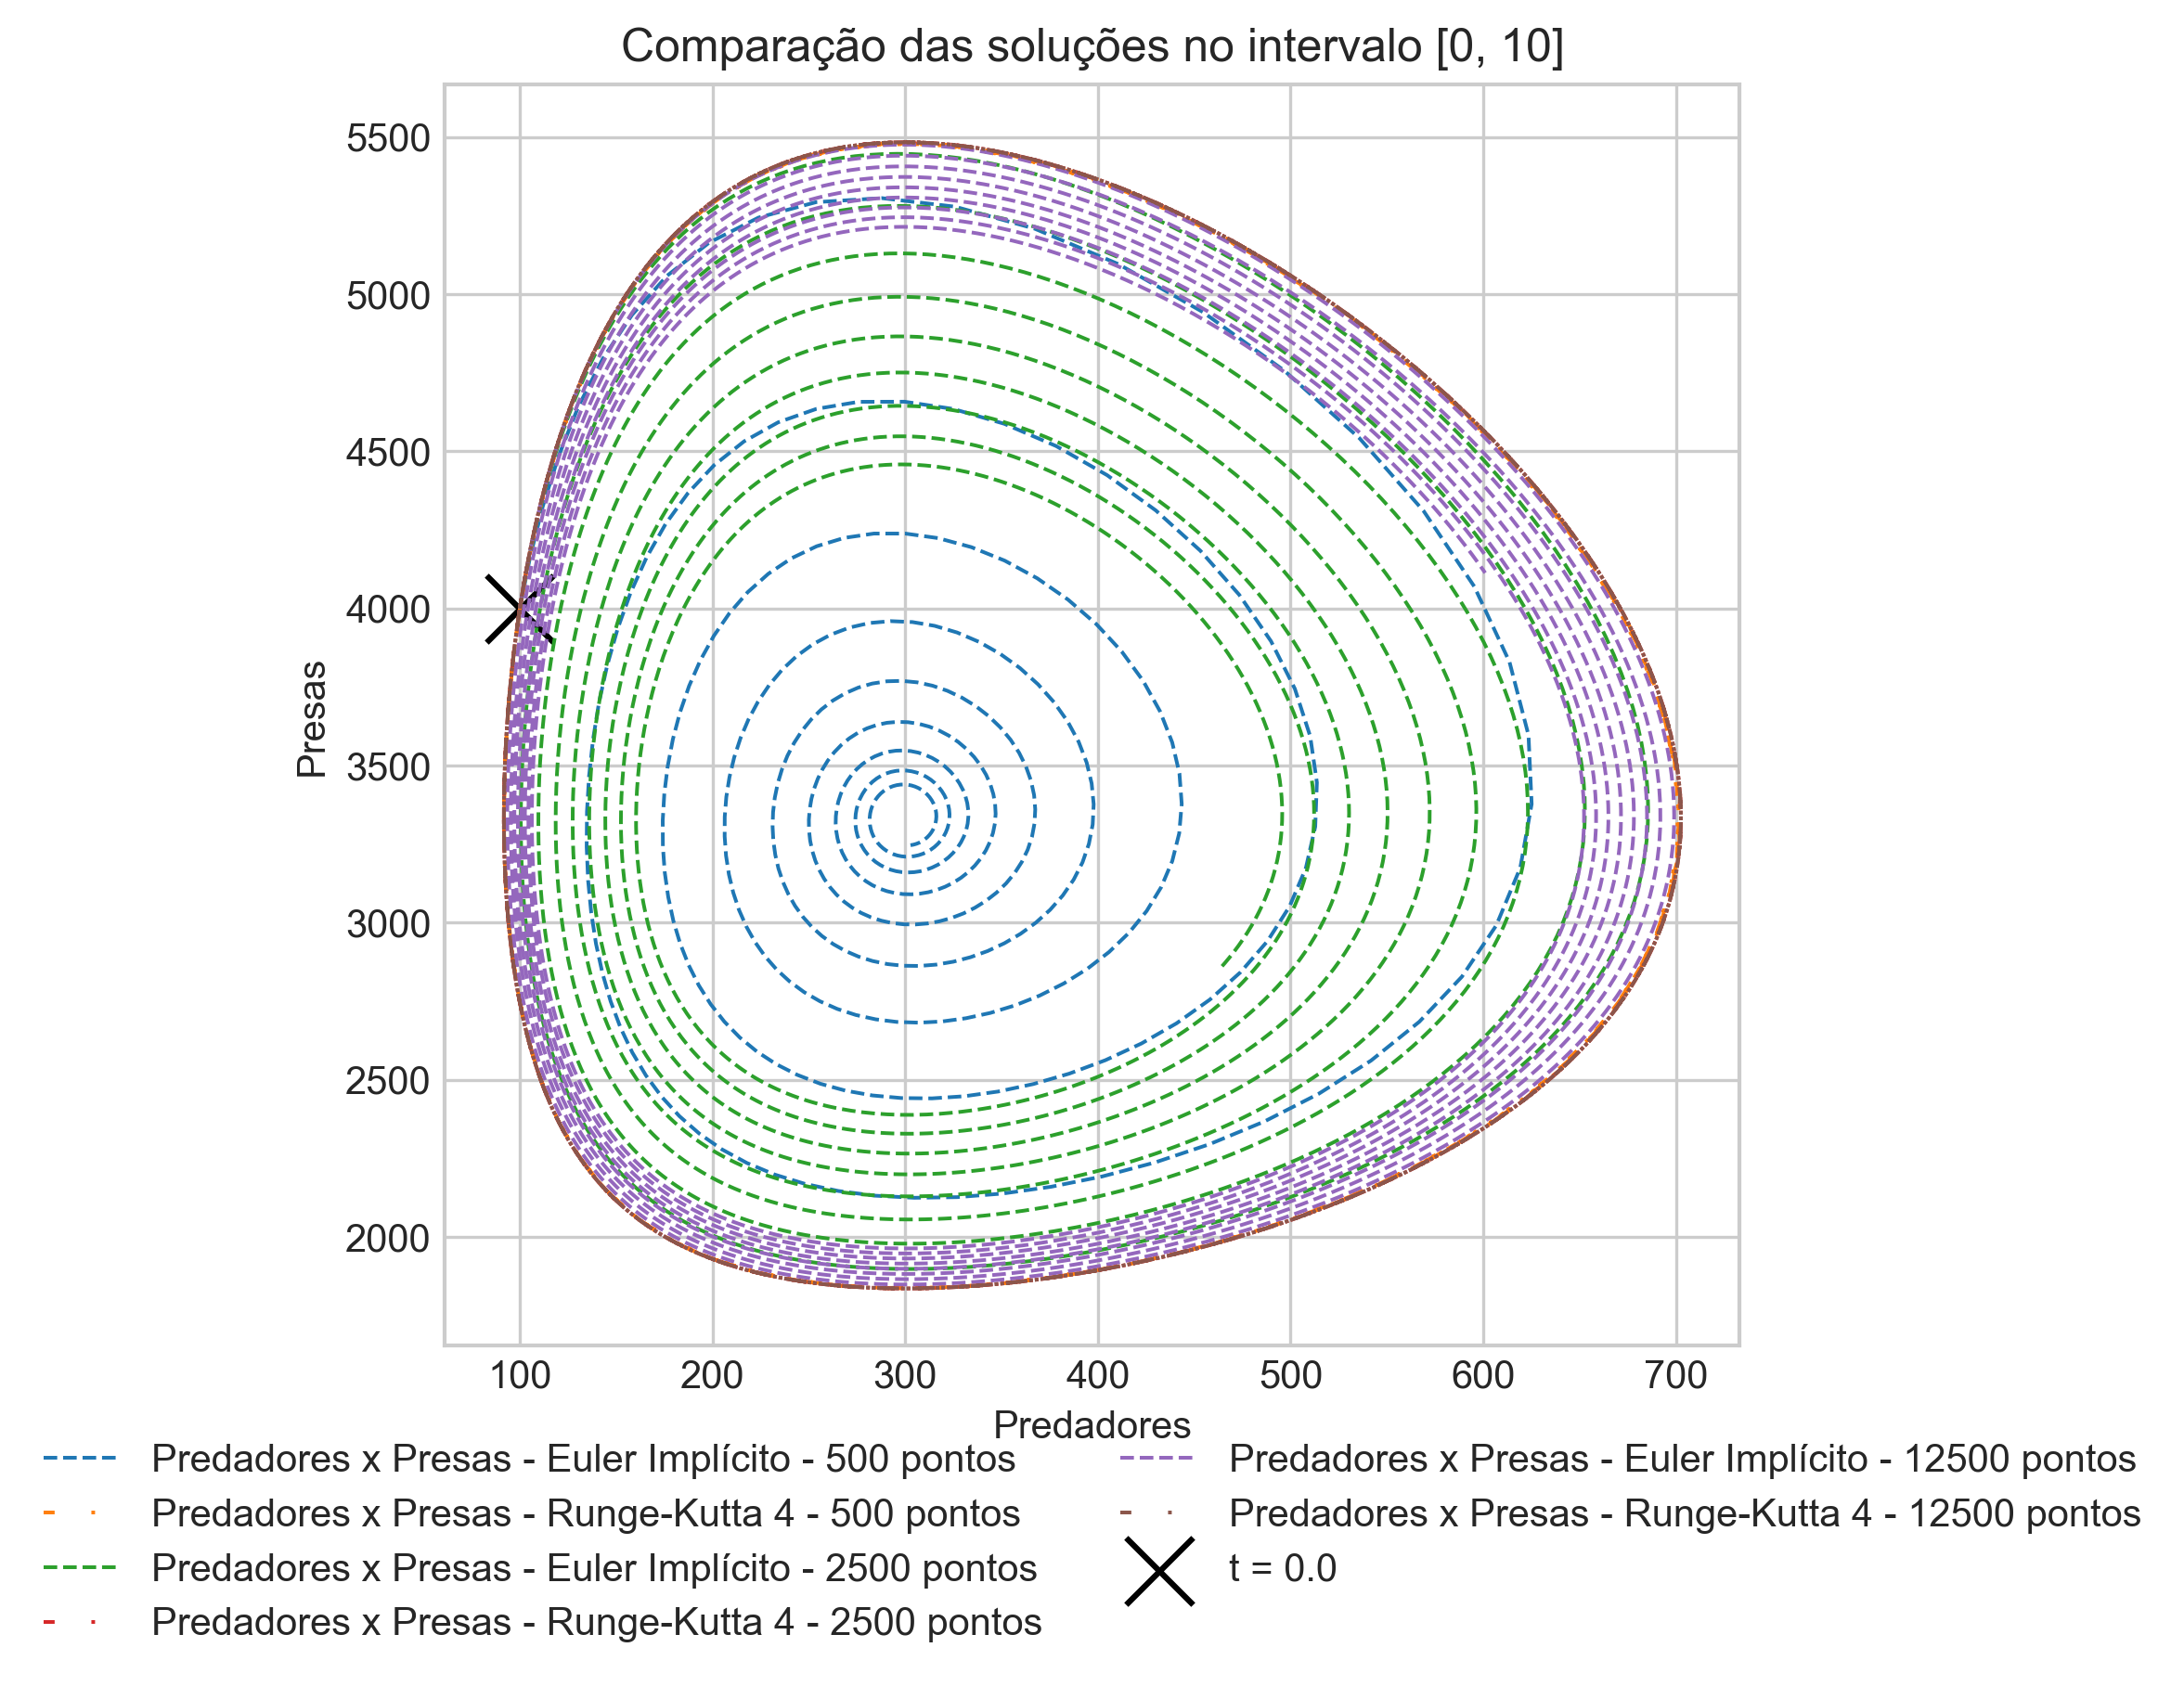
\includegraphics[height=10cm]{predator-prey/pp-comparison-2d.png}}
	}
   \mbox{
		\subfigure[]{
			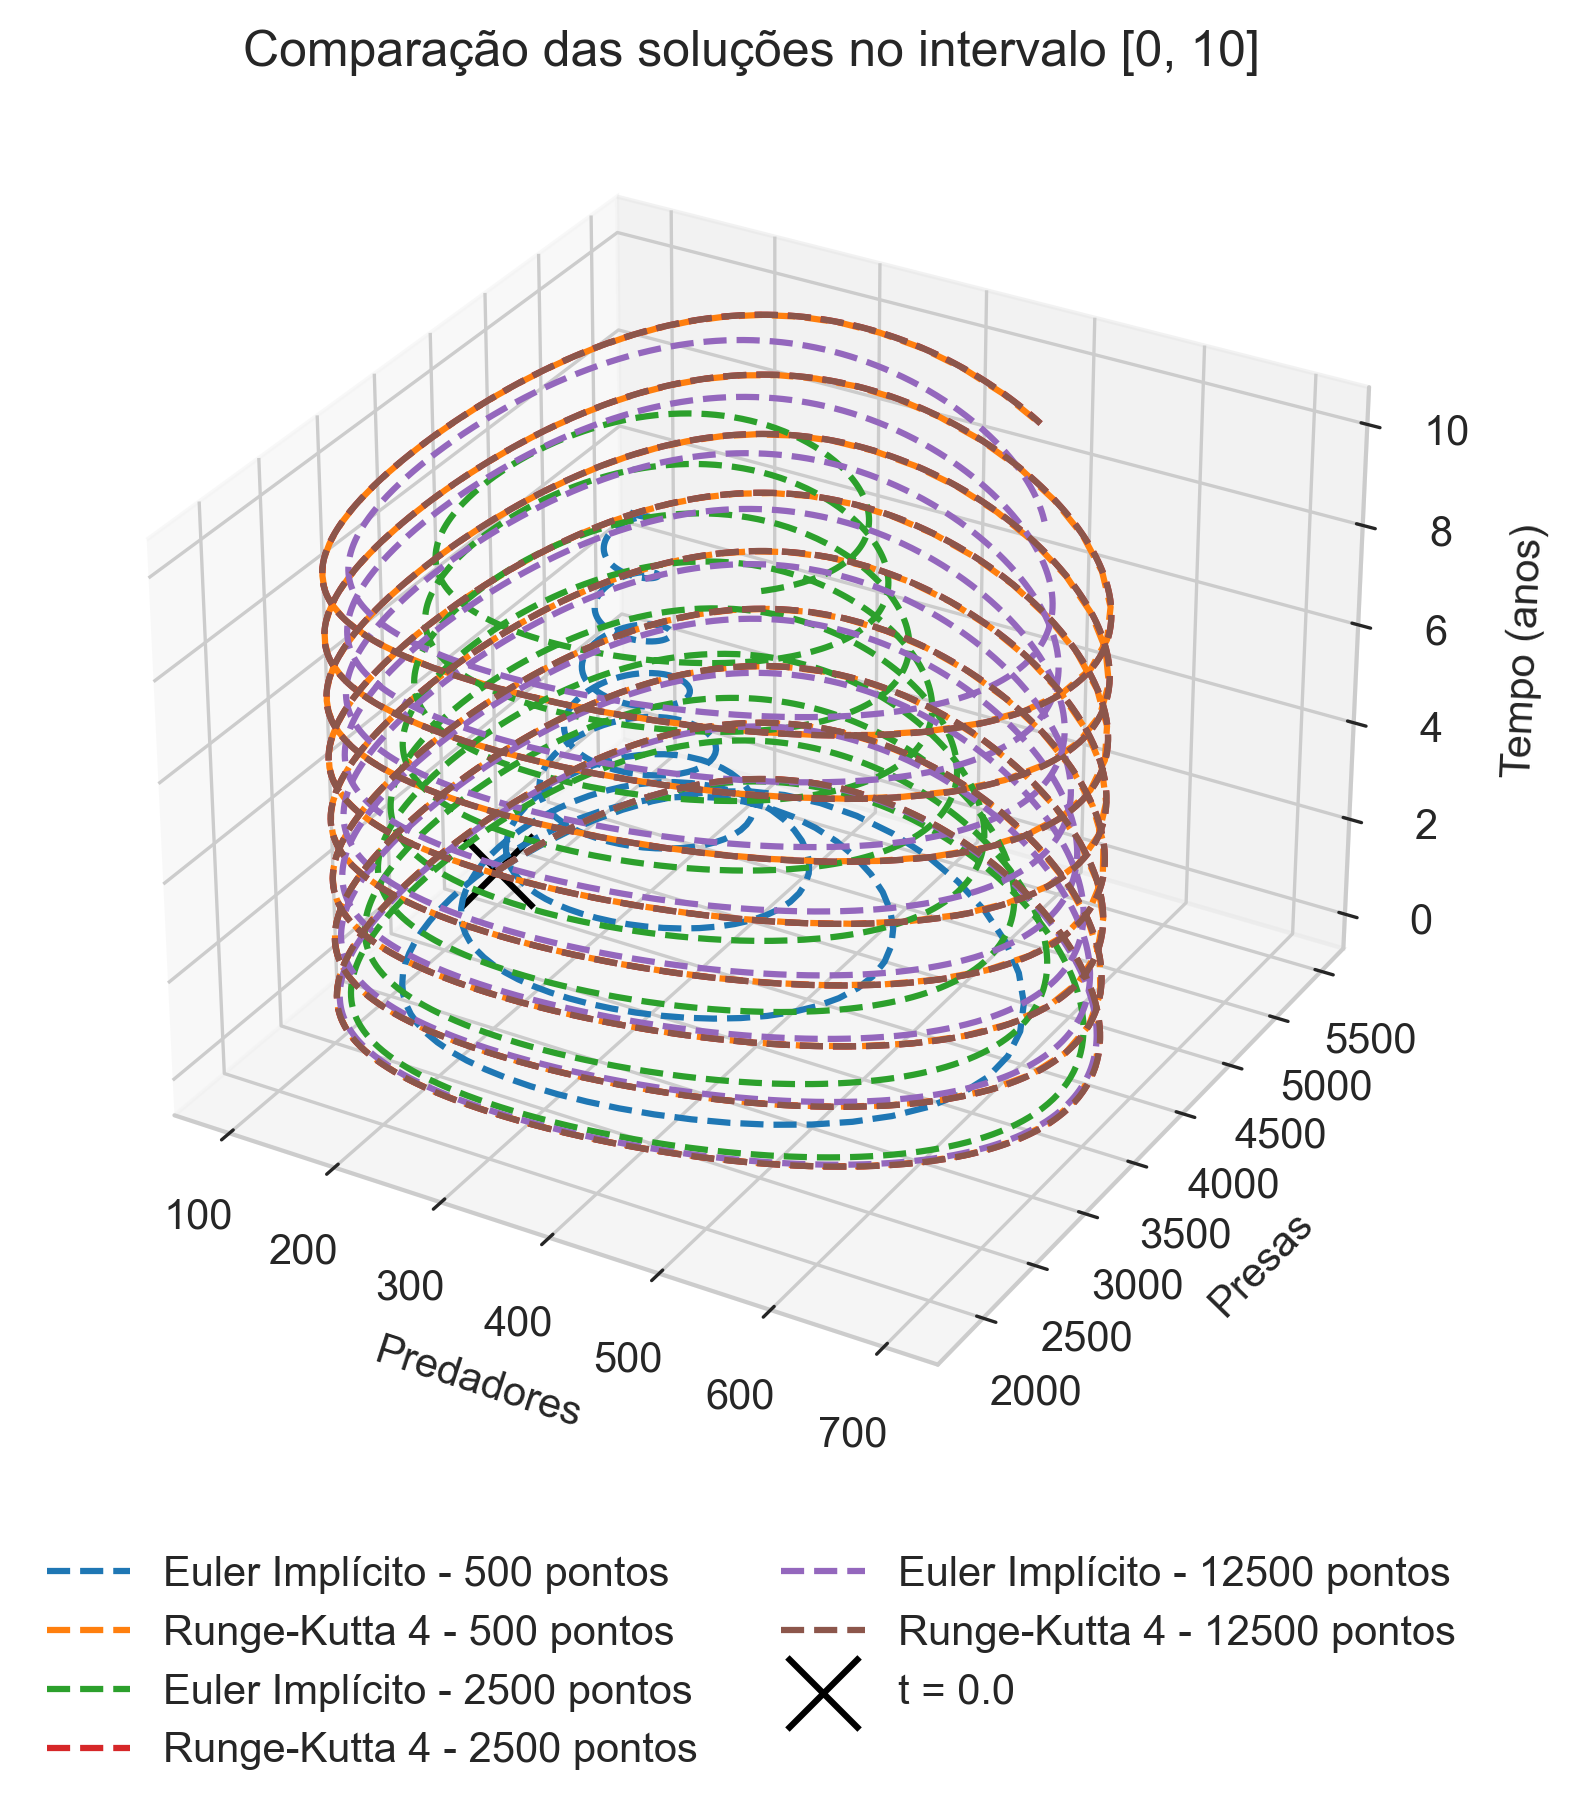
\includegraphics[height=10cm]{predator-prey/pp-comparison.png}}
   }
	\caption{(a) Representação bidimensional das soluções obtidas para distintas malhas; (b) Representação temporal das soluções obtidas}
    \label{img:comparison_plots}
\end{figure}

A Figura \ref{img:comparison_plots} mostra que o método de quarta ordem converge para a mesma solução, independentemente do refinamento da malha, evidenciando sua estabilidade e precisão numérica. Por outro lado, o método implícito apresentou maior sensibilidade ao refinamento da malha, tendo a solução se aproximado daquela obtida pelo método de Runge-Kutta. Apesar disso, o comportamento espiral ainda persiste no método implícito.

\begin{figure}[H]
	\centering
    \mbox{
        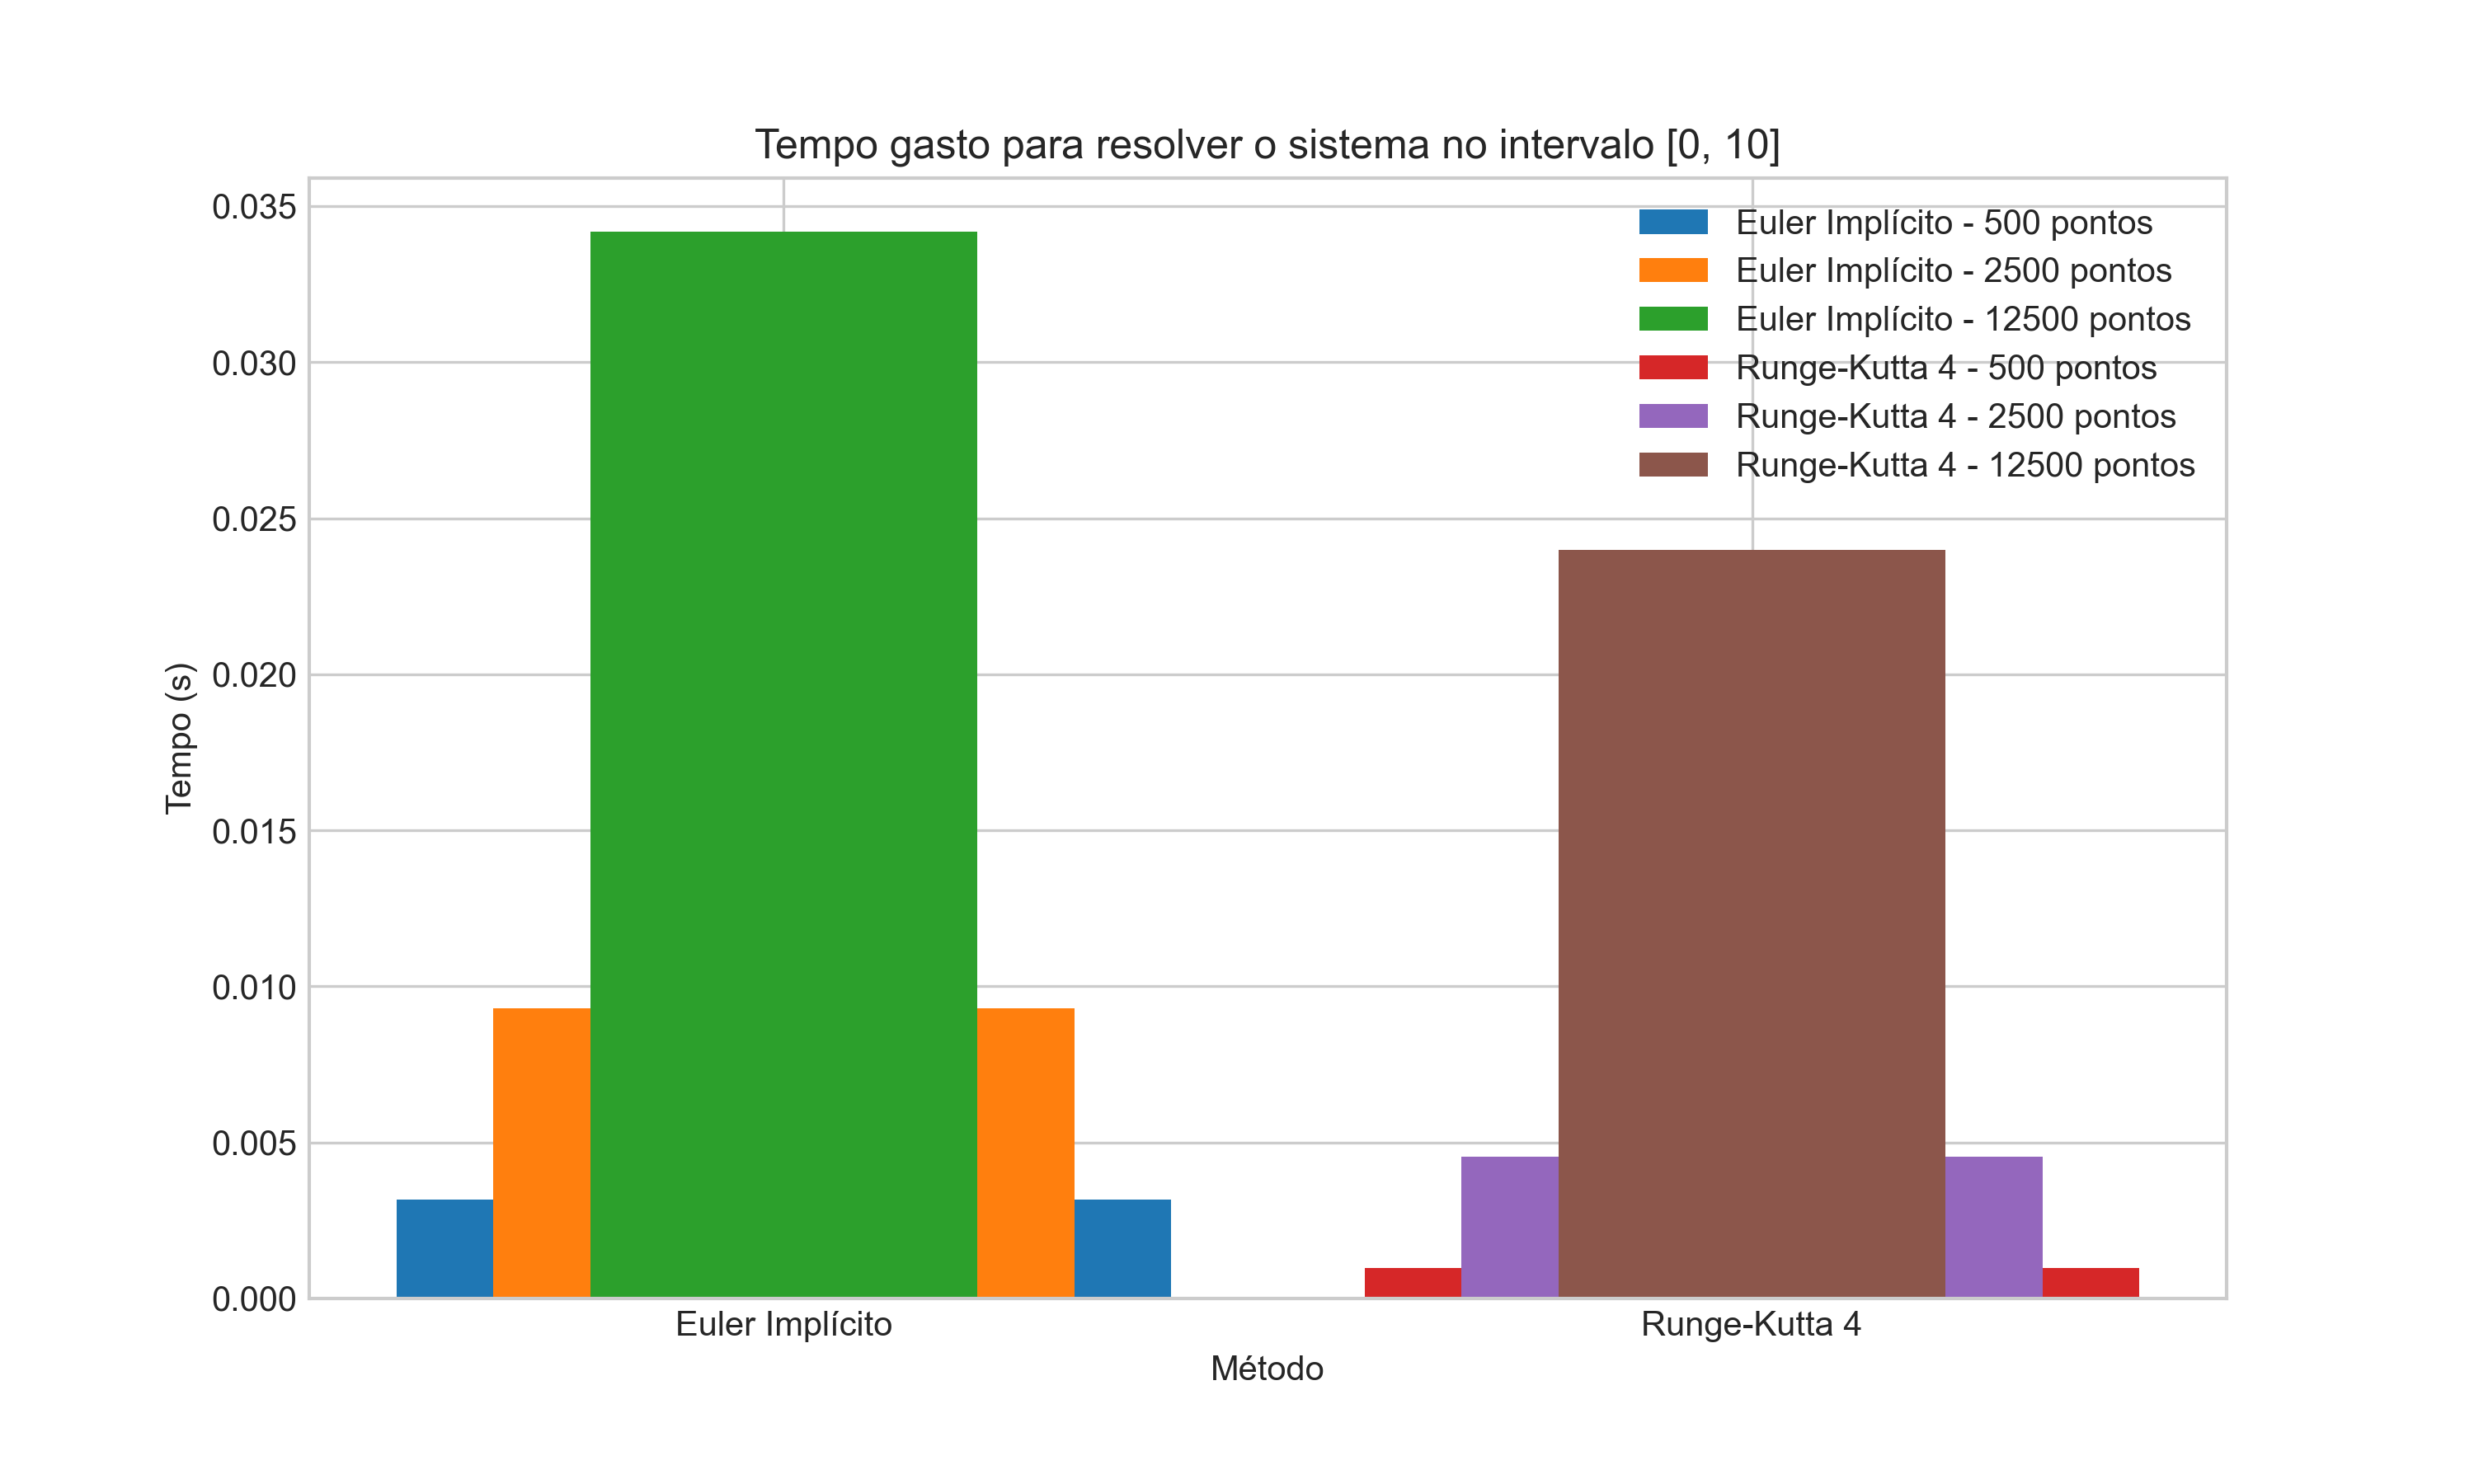
\includegraphics[width=14cm]{predator-prey/predator_prey-300dpi-time-comparison.png}
    }
	\caption{Tempo gasto para resolver o sistema.}
    \label{img:pp-times}
\end{figure}

Considerando a Figura \ref{img:comparison_plots}, é possível observar que ambos os métodos estão convergindo para a solução, porém, em velocidades distintas. É importante destacar que a escolha de um método dependerá da precisão e eficiência computacional desejadas. Nesse sentido, o método de quarta ordem pode ser considerado o mais adequado para este problema, uma vez que obteve uma solução melhor com uma quantidade de pontos bastante inferior ao método de primeira ordem, economizando tempo de processamento computacional, conforme apresentado na Figura \ref{img:pp-times}.
% \section{Considerações Finais}\label{sec:conclusion}



Este relatório apresentou a aplicação dos métodos computacionais de diferenças finitas e de Runge-Kutta para a análise temporal do crescimento de uma ou mais populações em um sistema fechado. Esses métodos oferecem uma alternativa vantajosa em relação à solução analítica, que nem sempre é conhecida ou de fácil cálculo.

Para otimizar o desempenho dos algoritmos, foi necessário recorrer à biblioteca de compilação \emph{Just-In-Time} devido à quantidade de tempo necessária para computar os $N$ pontos de cada problema. Além disso, foi utilizada uma escolha particular para resolver a equação implícita do método de Euler Implícito, que aumentou drasticamente o tempo de execução do método. No entanto, se a equação implícita fosse resolvida antes da execução, o tempo gasto em um problema genérico se aproximaria do tempo do método de Euler Explícito. Como evidenciado pelos gráficos apresentados neste trabalho, o método de Euler Implícito é o que consome mais tempo para ser completamente executado.

Em resumo, a aplicação dos métodos computacionais estudados neste trabalho permite o início de uma resolução de problemas complexos do mundo real, oferecendo uma alternativa eficiente e acessível para aproximar numericamente soluções que nem sempre são conhecidas ou de fácil cálculo.
% \input{acknowledgments.tex}
\section{Referências bibliográficas}
\begin{thebibliography}{99}
	
\bibitem{Bertalmio2000}
Bertalmio, M., Sapiro, G., Caselles, V., e Ballester, C. (2000). "Image inpainting". Proceedings of the 27th Annual Conference on Computer Graphics and Interactive Techniques — SIGGRAPH ’00.

\bibitem{Elharrouss2019}
Elharrouss, O., Almaadeed, N., Al-Maadeed, S., Akbari, Y. (2019). Image Inpainting: A Review. Neural Processing Letters.

\bibitem{Fontoura2022}
Fontoura, C. (2022). “Estudos De Métricas Para Quantificar Os Resultados De Aplicação De inpainting Para Melhoria Da Qualidade Do Processo De Extração De Feições Em Imagens Digitais”. Relatório de Qualificação de Doutorado, FCT-UNESP.

\bibitem{Dolhansky2018}
B. Dolhansky and C. C. Ferrer, "Eye In-painting with Exemplar Generative Adversarial Networks," 2018 IEEE/CVF Conference on Computer Vision and Pattern Recognition, 2018, pp. 7902-7911, doi: 10.1109/CVPR.2018.00824.

\bibitem{Bertalmio2001}
Bertalmio, M., Sapiro, G., Caselles, V.,  Ballester, C. (2001). Image inpainting. In Computer Graphics and Applications, 2001. Proceedings. 21st International Conference on (pp. 417-424). IEEE.

\bibitem{Criminisi2004}
Criminisi, A., Pérez, P., Toyama, K. (2004). Region filling and object removal by exemplar-based image inpainting. IEEE Transactions on image processing, 13(9), 1200-1212.

\bibitem{Efros1999}
Efros, A. A., Leung, T. K. (1999). Texture synthesis by non-parametric sampling. In Proceedings of the 26th annual conference on Computer graphicvs and interactive techniques (pp. 1033-1038). ACM.


\end{thebibliography}


\end{document}


